% !TeX root = 00-main.tex
%% ---------------------------------------------------------------------
%% Appendix C: Extended implementation and supplementary results.
%% All numbers reconciled to the authoritative v2lowrank_source run and verified against:
%%   results_hpc/ude/{Re_per_program,ladder,transport_stability,d_rho_summary,dataset_folds}_*.{parquet,json}
%%   results_hpc/panin/{Re_per_program,ladder,dataset_folds,Re_by_fold/*}
%%   workflow/config.yaml, workflow/config_{aah_ais,ais_invasive}.yaml, workflow/envs/crrt.yaml,
%%   crrt/ude/{context.py,coupling.py,field.py}, outputs/*/w_context_channels.json.
%%  marks anything not verifiable from a file (see report). Compilable with the
%% packages already loaded by 00-main.tex (booktabs, longtable, graphicx, xcolor); no new packages.
%% The \appendix + \makeatletter block in 11-appendix-A.tex precedes this chapter; do NOT repeat it.
%% ---------------------------------------------------------------------

\chapter{Extended Implementation and Supplementary Results}\label{chap:appendix-c}

This appendix records the implementation detail and the full supplementary tables behind the
results of Chapter~\ref{chap:results}. Every numerical value is reconciled to the authoritative
\texttt{v2lowrank\_source} run---low-rank identifiable self-field (rank $32$) with source-fixed
context timing $w(\tau)=w_i$---so that the main-text figures and the tables here derive from a single
set of trained fields. The material is organized as ten sections: the symbol index for
Chapter~\ref{chap:methods} (C.1); the data, feature, and configuration inventory (C.2); the fitting
diagnostics (C.3); the complete falsification ladders for both LUAD edges (C.4); the
program-stability atlas (C.5); the spatial niche-association analysis (C.6); the invasion-edge
supplement (C.7); the co-expression and regulon corroboration (C.8); the PanIN supplement (C.9); and
the software and reproducibility manifest (C.10).

% =====================================================================
\section{Symbol index}\label{sec:app-c-symbols}

Table~\ref{tab:app-c-symbols} lists every symbol appearing in the numbered
equations of Chapter~\ref{chap:methods}, together with the equations in which
each occurs. Equation numbers refer to the sequential numbering of
Chapter~\ref{chap:methods}. Symbols that recur across several sections are also
collected in the notation table of Section~\ref{sec:methods-notation}; this
index additionally covers symbols local to a single equation, which are defined
at their point of use in the text but are gathered here for reference.
Dimensions are those of the frozen LUAD analysis matrix.

\begin{longtable}{@{}>{$}l<{$}p{0.19\textwidth}p{0.42\textwidth}p{0.15\textwidth}@{}}
\caption{Every symbol appearing in the numbered equations of
Chapter~\ref{chap:methods}, with the equations in which it occurs.}
\label{tab:app-c-symbols}\\
\toprule
\textrm{Symbol} & Type / dimension & Meaning & Equations \\
\midrule
\endfirsthead
\multicolumn{4}{l}{\small\itshape Table~\ref{tab:app-c-symbols} continued from previous page}\\
\toprule
\textrm{Symbol} & Type / dimension & Meaning & Equations \\
\midrule
\endhead
\midrule
\multicolumn{4}{r}{\small\itshape continued on next page}\\
\endfoot
\bottomrule
\endlastfoot

\multicolumn{4}{l}{\textit{Indices and sets}}\\
\addlinespace[0.2em]
i,\;j & index & source, target receiver & most \\
k,\;\ell & index & regulatory coordinate & 19, 30 \\
c & $\in\{1,\ldots,K\}$ & ecological stratum & 11--15, 33, 34 \\
f & index & cross-validation fold & 7, 33--35 \\
d,\;s & label & donor, pathological stage & 6, 7, 32, 38 \\
e & label & epithelial lineage & 3 \\
g & index & gene & 3 \\
K & $3$ (LUAD), $2$ (PanIN) & number of ecological strata & 11 \\
\mathcal{S},\;\mathcal{T} & sets & source-, target-stage receivers & 8, 12, 39, 43 \\
\mathcal{E} & set & epithelial reference populations & 2 \\
\mathcal{P} & $\subset\{1,\ldots,d_z\}$ & pathway-coordinate indices & 19 \\
\mathcal{C}_f^{\mathrm{eval}} & set & strata with held-out common support & 34 \\
\mathcal{D} & set & the model-ready dataset & 6 \\
\mathcal{B}_{\mathrm{src}} & set & sampled source batch & 43 \\
\mathcal{T}^{(1)},\mathcal{T}^{(2)} & sets & two independent target subsamples & 42, 43 \\

\midrule
\multicolumn{4}{l}{\textit{Dimensions and counts}}\\
\addlinespace[0.2em]
d_z & $773$ & regulatory state dimension & 4, 16, 20, 29, 39 \\
d_w & $35$ & context dimension after leakage exclusions & 5 \\
d_r & $14$ & pathway coordinates (the context bottleneck) & 18, 21 \\
r_A & $32$ & rank bound on $A$ & 20 \\
N & count & receivers in $\mathcal{D}$ & 6 \\
N_d,\;N_{ds} & count & receivers per donor; per donor and stage & 32, 38 \\
N_f & count & held-out source receivers in fold $f$ & 39 \\
n_c,\;m_c & count & source, target receivers in stratum $c$ & 14 \\
n_{\min},\;D_{\min} & $10$, $2$ & common-support thresholds & 12 \\
D_f & count & evaluated donors in fold $f$ & 35 \\
D_{\mathrm{eval}} & count & evaluated source-stage donors & 32 \\

\midrule
\multicolumn{4}{l}{\textit{Data and state}}\\
\addlinespace[0.2em]
z_i^{\mathrm{obs}} & $\mathbb{R}^{d_z}$ & observed receiver state & 1, 4, 6, 13, 16, 23, 24, 39 \\
z(\tau) & $\mathbb{R}^{d_z}$ & state at progression coordinate $\tau$ & 17 \\
z_\tau & $\mathbb{R}^{d_z}$ & linear interpolant between a pair & 25, 26 \\
\overline{z} & $\mathbb{R}^{d_z}$ & pathway-masked state & 18, 19, 23, 40 \\
z_i^{\mathrm{full}}(1) & $\mathbb{R}^{d_z}$ & endpoint, context branch active & 1, 29, 31 \\
z_i^{\mathrm{self}}(1) & $\mathbb{R}^{d_z}$ & endpoint, context branch inactive & 1, 24, 29, 31 \\
p_i,\;t_i & $\mathbb{R}^{14}$, $\mathbb{R}^{759}$ & pathway, TF blocks of $z$ & 4 \\
w_i & $\mathbb{R}^{d_w}$ & ecological context & 1, 5, 6, 22, 23, 31, 38 \\
q_i,\;h_i & --- & composition, neighborhood blocks of $w$ & 5 \\
\overline{w}_{ds} & $\mathbb{R}^{d_w}$ & donor--stage-average context & 38 \\
u_i & $\mathbb{R}^{2}$ & coarse CAF/immune composition & 9, 10, 11 \\
a_i^{\mathrm{epi}} & $[0,1]$ & epithelial abundance of spot $i$ & 2, 6 \\
x_{ig}^{\mathrm{log}} & scalar & log-normalized decoded expression & 3 \\
\widehat{\pi}_{i\ell} & $[0,1]$ & DestVI proportion of population $\ell$ & 2 \\
\tau & $[0,1]$ & normalized progression coordinate & 17, 18, 21--26, 31 \\
\Delta z_{ij} & $\mathbb{R}^{d_z}$ & observed pair displacement & 16 \\

\midrule
\multicolumn{4}{l}{\textit{Model parameters}}\\
\addlinespace[0.2em]
A & $\mathbb{R}^{d_z\times d_z}$ & linear state-to-velocity operator, rank $\leq r_A$ & 18, 20, 23, 40 \\
U,\;V & $\mathbb{R}^{d_z\times r_A}$, $\mathbb{R}^{r_A\times d_z}$ & factors of $A$; individually unidentifiable & 20 \\
b & $\mathbb{R}^{d_z}$ & intercept (state-independent drift) & 18, 23, 40 \\
B & $\mathbb{R}^{d_z\times d_r}$ & maps pathway activity into full velocity & 18, 23, 40 \\
G & $\mathbb{R}^{d_r\times d_w}$ & context gate weights & 21, 23, 40 \\
b_g & $\mathbb{R}^{d_r}$ & context gate bias & 21, 23, 40 \\
M_{\mathrm{ctx}} & $\mathbb{R}^{d_z\times d_r}$ & expands gated pathway signal to full velocity & 21, 23, 40 \\
\rho_s & neural network & self nonlinear residual field & 18, 23, 40 \\
\rho_c & neural network & context nonlinear residual field & 21, 23, 40 \\
\theta & --- & all trainable parameters collectively & 26 \\

\midrule
\multicolumn{4}{l}{\textit{Operators and fields}}\\
\addlinespace[0.2em]
r(z) & $\mathbb{R}^{d_z}\!\to\!\mathbb{R}^{d_r}$ & selects the pathway coordinates & 18, 21, 40 \\
\gamma(w) & $[-1,1]^{d_r}$ & bounded per-pathway context modulation & 21 \\
\odot & --- & element-wise (Hadamard) product & 21, 23, 40 \\
\oslash & --- & element-wise division & 10 \\
v_{\mathrm{self}} & $\mathbb{R}^{d_z}$ & intrinsic velocity branch & 17, 18, 24, 31 \\
v_{\mathrm{context}} & $\mathbb{R}^{d_z}$ & context velocity branch & 17, 21, 31 \\
v_{\mathrm{full}} & $\mathbb{R}^{d_z}$ & their sum, the fitted field & 17 \\
v_{\mathrm{structured}} & $\mathbb{R}^{d_z}$ & all non-neural terms & 40, 41 \\
v_{\mathrm{neural}} & $\mathbb{R}^{d_z}$ & $\rho_s+\rho_c$ & 40, 41 \\
a(u_i) & function & frozen fold-fitted stratifier & 11 \\
f(i) & function & fold assigned to receiver $i$ & 7 \\
T_{1},\;T_{2} & $\mathbb{R}^{d_z}$ & barycentric targets under two subsamples & 42, 43 \\

\midrule
\multicolumn{4}{l}{\textit{Transport}}\\
\addlinespace[0.2em]
\Pi_c^{\ast} & $\mathbb{R}^{n_c\times m_c}$ & entropic transport plan within stratum $c$ & 14, 15 \\
\Pi^{(1)}_{ij} & scalar & transport mass, source $i$ to target $j$ & 42 \\
C_{ij} & scalar & transport cost $\lVert z_i-z_j\rVert_2^2$ & 13, 14 \\
\varepsilon & $0.05$ & entropic regularization strength & 14, 33 \\
\alpha_i,\;\beta_j & $1/n_c$, $1/m_c$ & uniform empirical marginals & 14 \\
\mathcal{U}(\alpha,\beta) & set & plans with those marginals & 14 \\
\eta_i & scalar & ecological score (first PC of $u$) & 10 \\
c_i & $\in\{1,\ldots,K\}$ & assigned stratum & 11 \\
b_1 & $\mathbb{R}^{2}$ & first PCA loading vector & 10 \\
\mu_u,\;\sigma_u & $\mathbb{R}^{2}$ & training-fold mean, SD of $u$ & 10 \\

\midrule
\multicolumn{4}{l}{\textit{Estimand and evaluation}}\\
\addlinespace[0.2em]
R_{\mathrm{cond},i} & $\mathbb{R}^{d_z}$ & the estimand: per-receiver context residual & 1, 29, 31 \\
R_{\mathrm{cond},ik} & scalar & the same, at coordinate $k$ & 30 \\
\overline{R}_{\mathrm{cond},d} & $\mathbb{R}^{d_z}$ & donor-mean residual & 32 \\
\overline{R}_{\mathrm{cond}} & $\mathbb{R}^{d_z}$ & equal-donor cohort residual & 32 \\
\overline{R}_{fk}^{\ast(b)} & scalar & bootstrap replicate $b$, fold $f$, program $k$ & 35 \\
D_{\mathrm{OT},fc} & scalar & per-stratum endpoint Sinkhorn cost & 33 \\
D_{\mathrm{OT},f}^{\mathrm{conditional}} & scalar & primary endpoint metric & 34 \\
\omega_{fc} & $[0,1]$ & source-mass weight of stratum $c$ & 34 \\
n_{fc}^{\mathrm{src}} & count & held-out source receivers in stratum $c$ & 34 \\
\widehat{Z}_{1,f},\;Z_{\mathrm{tgt},f} & sets & predicted, observed target populations & 33 \\
\mathcal{L}_{\mathrm{CFM}} & scalar & flow-matching loss & 26, 27 \\
\mathcal{L}^{(\mathrm{C})} & scalar & Stage C composite objective & 27 \\
\lambda_{\bullet} & scalars & the five loss weights & 27, 28 \\
\operatorname{MSE}_{\mathrm{recon}} & scalar & leakage-audit reconstruction error & 39 \\
D_{\rho} & scalar & neural-to-structured velocity ratio & 41 \\
D_N & scalar & transport matching-stability & 43, 44 \\
\widehat{\Sigma}_{\mathrm{tgt}} & matrix & empirical target-state covariance & 44 \\

\midrule
\multicolumn{4}{l}{\textit{Synthetic benchmark only}}\\
\addlinespace[0.2em]
\Phi_{\mathrm{self}} & function & planted intrinsic transformation & 45 \\
R_i^{\mathrm{true}} & vector & planted context displacement (ground truth) & 45 \\
\xi_i & vector & Gaussian noise, SD $0.1$ & 45 \\
\mathcal{G}_{\mathrm{context}} & scalar & context-gain statistic & 46 \\
\mathrm{Var}_{\mathrm{self}},\mathrm{Var}_{\mathrm{full}} & scalar & residual variances of the two fits & 46 \\

\end{longtable}

Four symbol pairs were deliberately kept distinct to avoid collision:
$\varepsilon$ (transport regularization) against $\xi$ (synthetic noise);
$V$ (a factor of $A$) against $\mathrm{Var}_{\bullet}$ (residual variances);
$G$ (gate weights) against $\mathcal{G}_{\mathrm{context}}$ (the gain
statistic); and $T_{1},T_{2}$ (barycentric targets) against
$\Phi_{\mathrm{self}}$ (the synthetic transformation). Likewise $B$ (the
pathway map) is distinct from the batch sizes $B_{\mathrm{OT}}$ and
$B_{\mathrm{pair}}$.

% =====================================================================
\section{Data, features, and configuration}\label{sec:app-c-config}

This section collects the exact inputs and settings behind every fitted model:
the cohorts and their sizes, the quality-control thresholds, the regulatory and
context feature definitions, the patient-fold partition, the edge-selector
configurations, and the complete hyperparameter and seed table. Together these
specify what the model saw and how it was fitted.

\subsection{Dataset inventory}\label{sec:app-c-inventory}

The primary cohort is the LUAD progression series (single-nucleus RNA, GEO accession GSE308103),
spanning five morphological stages, paired with matched spatial transcriptomics of the same
specimens (GEO accession GSE307534). Cell-type reference transfer uses the Lung Cancer Atlas (LuCA, disease-aware, primary)
and the Human Lung Cell Atlas (HLCA, ablation reference). The transferability probe is a graded
pancreatic intraepithelial neoplasia (PanIN) Visium series (GEO accession GSE254829, seven slides)
decoded against the PDAC single-nucleus atlas (GEO accession GSE202051).


Table~\ref{tab:app-c-inventory} gives the per-stage donor and epithelial-receiver counts. Donor
coverage per stage is 23 Normal, 10 AAH, 12 AIS, 4 MIA, and 25 LUAD.

\begin{table}[htbp]
  \centering
  \caption[LUAD dataset inventory]{LUAD dataset inventory. Donor counts per stage and epithelial
  receiver counts, from the edge-support manifest. Epithelial-cell counts are the numbers entering
  transport on the edge that uses each stage as source or target.}
  \label{tab:app-c-inventory}
  \begin{tabular}{lcc}
    \toprule
    Stage & Donors & Epithelial cells \\
    \midrule
    Normal & 23 & 48{,}295 \\
    AAH    & 10 & 29{,}712 \\
    AIS    & 12 & 48{,}688 \\
    MIA    & 4  & 8{,}356 \\
    LUAD   & 25 & 144{,}226 \\
    \bottomrule
  \end{tabular}
\end{table}

\subsection{Preprocessing thresholds}\label{sec:app-c-preproc}

Quality control and feature selection were applied uniformly across all datasets before typing and
regulatory scoring. Cells were retained with at least $200$ detected genes and at most $20\%$
mitochondrial counts; genes expressed in fewer than $3$ cells were dropped; and $3000$ highly
variable genes were selected (Seurat v3 flavor) for the reference-mapping and typing steps.
These thresholds are listed in Table~\ref{tab:app-c-qc}.

\begin{table}[htbp]
  \centering
  \caption[Preprocessing thresholds]{Quality-control and feature-selection thresholds, applied
  identically to the LUAD and PanIN inputs.}
  \label{tab:app-c-qc}
  \begin{tabular}{ll}
    \toprule
    Threshold & Value \\
    \midrule
    Minimum genes per cell        & $200$ \\
    Maximum mitochondrial percent & $20\%$ \\
    Minimum cells per gene        & $3$ \\
    Highly variable genes         & $3000$ (Seurat v3) \\
    \bottomrule
  \end{tabular}
\end{table}

\subsection{Regulatory feature list}\label{sec:app-c-regfeatures}

The receiver regulatory state $z \in \mathbb{R}^{d_z}$ has dimension $d_z = 773$ on the LUAD edges:
$14$ PROGENy pathway activities and $759$ CollecTRI transcription-factor regulon activities, each
scored with decoupleR. The $14$ PROGENy pathways are: Androgen, EGFR, Estrogen, Hypoxia, JAK-STAT,
MAPK, NF$\kappa$B, PI3K, TGF$\beta$, TNF$\alpha$, Trail, VEGF, WNT, and p53. The first $d_r = 14$
coordinates (the pathway sub-vector) are the interpretable sub-space over which the pathway-level
$R_{\mathrm{cond}}$ effects of Chapter~\ref{chap:results} are reported. The $759$ transcription-factor
programs are named \texttt{tf\_<SYMBOL>} and are not enumerated here; the complete indexed program
list, with per-program mean $R_{\mathrm{cond}}$, held-out confidence interval, and stability class,
is provided in the machine-readable program tables (\texttt{Re\_per\_program\_<edge>\_v2lowrank\_source.parquet}
and the dossier CSVs). On the PanIN edge the same construction yields $762$ programs
($14$ PROGENy pathways $+$ $748$ transcription factors); the transcription-factor count is smaller
because regulons with insufficient target support in the pancreatic data are dropped at scoring time.

\subsection{Context feature list}\label{sec:app-c-ctxfeatures}

The niche-context vector $w$ is assembled per receiver from the spatial pipeline and then passed
through the anti-leakage strip (\texttt{crrt/ude/context.py}), which removes every receiver-derived
channel---epithelial composition fractions, whole-spot regulatory programs
(\texttt{pathway\_*}/\texttt{tf\_*}), malignant fraction, diversity, stage, and donor identity---so
that the context can carry no copy of the outcome it is used to explain. What remains are three
channel types: (i) two broad same-spot ecology fractions, \texttt{caf\_fraction} and
\texttt{immune\_fraction}; (ii) non-epithelial cell-type composition fractions (\texttt{comp\_*});
and (iii) six neighborhood aggregates \texttt{ctx\_0}--\texttt{ctx\_5} computed by the Merchavit
spatial backend (a Rust reimplementation of the BANKSY neighborhood algorithm). On the LUAD invasion
edge the retained context vector has dimension $d_w = 35$: two fraction channels, $27$ non-epithelial
\texttt{comp\_*} LuCA cell types (B cell, CD4/CD8 T cell, regulatory T cell, natural killer cell,
several dendritic-cell and monocyte subsets, alveolar macrophage, macrophage, myeloid cell,
neutrophil, mast cell, plasma cell, lung/bronchus fibroblast, mesothelial cell, stromal cell,
smooth-muscle cell, pericyte, and capillary/vein/lymphatic/pulmonary-artery endothelial cells), and
the six \texttt{ctx\_*} neighborhood channels. The AAH$\rightarrow$AIS edge uses the identical schema.
On the PanIN edge $d_w = 16$: two fraction channels, eight non-epithelial PDAC-atlas
\texttt{comp\_*} types (Adipocyte, Cancer-associated fibroblast, Endothelial, Lymphoid, Myeloid,
Pericyte, Schwann, Vascular smooth muscle), and the six \texttt{ctx\_*} channels.

Critically, the coupling that supervises training is stratified on a still narrower coarse-niche
allowlist $a(w)$ to protect the estimand from circularity: only the broad non-epithelial fractions
(\texttt{caf\_fraction}, \texttt{immune\_fraction}, and---in the fuller allowlist---\texttt{myeloid},
\texttt{stromal}, \texttt{lymphoid}, and \texttt{endothelial} fractions) are admissible for
stratification. The primary run stratifies on \texttt{caf\_fraction} and \texttt{immune\_fraction}.

\subsection{Patient-fold assignments}\label{sec:app-c-folds}

All CRRT-UDE estimates use patient-held-out cross-validation: every receiver from a given donor is
assigned to a single fold, so no donor contributes to both training and evaluation. The frozen niche
stratifier and the optimal-transport coupling are fit on training donors only and applied to
held-out donors. Table~\ref{tab:app-c-folds} gives the donor-to-fold assignment for each LUAD edge
and for the PanIN edge. The AAH$\rightarrow$AIS edge uses five folds over $20$ donors (four donors
per fold); the AIS$\rightarrow$invasive edge uses five folds over $25$ donors (fold sizes
$6,6,5,4,4$); the PanIN edge uses three folds over the seven slides.

\begin{table}[htbp]
  \centering
  \caption[Patient-fold assignments]{Donor-to-fold assignments (patient-held-out cross-validation).
  Each donor is assigned to exactly one held-out fold. LUAD donors are labelled P1--P25; PanIN
  donors are the seven Visium slides.}
  \label{tab:app-c-folds}
  \footnotesize
  \begin{tabular}{@{}llp{0.52\textwidth}@{}}
    \toprule
    Edge & Fold & Held-out donors \\
    \midrule
    AAH$\rightarrow$AIS      & 0 & P8, P9, P11, P14 \\
    ($5$ folds, $20$ donors) & 1 & P20, P21, P23, P25 \\
                             & 2 & P1, P4, P12, P19 \\
                             & 3 & P16, P17, P22, P24 \\
                             & 4 & P2, P3, P5, P6 \\
    \midrule
    AIS$\rightarrow$invasive & 0 & P13, P15, P19, P20, P21, P23 \\
    ($5$ folds, $25$ donors) & 1 & P1, P3, P5, P8, P11, P18 \\
                             & 2 & P2, P9, P10, P17, P25 \\
                             & 3 & P6, P7, P12, P16 \\
                             & 4 & P4, P14, P22, P24 \\
    \midrule
    PanIN LG$\rightarrow$HG  & 0 & PanIN-HG4, PanIN-LG2, PanIN-LG3 \\
    ($3$ folds, $7$ slides)  & 1 & PanIN-HG2, PanIN-HG3 \\
                             & 2 & PanIN-HG1, PanIN-LG1 \\
    \bottomrule
  \end{tabular}
\end{table}

\subsection{Edge-selector configurations}\label{sec:app-c-edges}

The transport edge is selected by a dedicated configuration file layered on top of the shared base
configuration, so that an ordinary pipeline invocation can never silently run the wrong edge. Each
selector sets the three \texttt{primary\_edge} keys explicitly: \texttt{source}, \texttt{target}, and
\texttt{target\_members}. The AAH$\rightarrow$AIS selector sets \texttt{source: AAH},
\texttt{target: AIS}, \texttt{target\_members: [AIS]} (no pooling; a plain single-stage edge). The
invasion selector sets \texttt{source: AIS}, \texttt{target: invasive},
\texttt{target\_members: [MIA, LUAD]}, which pools the raw MIA and LUAD stages into a single
``invasive'' target label at ingest (few MIA specimens are combined with LUAD). The PanIN block sets
\texttt{source: low\_grade}, \texttt{target: high\_grade}. Setting \texttt{target\_members} equal to
\texttt{[target]} is the sentinel for ``no pooling,'' which keeps the single-stage edges byte-identical
to the unpooled pipeline.

\subsection{Hyperparameters and seeds}\label{sec:app-c-hyperparams}

Table~\ref{tab:app-c-hyperparams} records every hyperparameter of the CRRT-UDE model and its training
schedule, exactly as set in the run configuration. The self field uses a low-rank identifiable linear
map $A = UV^{\top}$ of rank $32$ ($2\,d_z\,r = 2\cdot773\cdot32 \approx 49{,}500$ parameters, defensible
on the order of $25$ donors, versus $\sim\!600{,}000$ for a full-rank $773\times773$ map). Training is
the three-stage schedule of Appendix~\ref{chap:appendix-b}: Stage~A fits the self field
($1000$ steps, learning rate $10^{-3}$), Stage~B fits the frozen-self context residual
($500$ steps, $10^{-3}$), and Stage~C jointly refines under the anchor penalty
($500$ steps, $10^{-4}$). Trajectories are integrated by a fourth-order Runge--Kutta scheme with
$4$ steps. The global seed is $0$; per-fold and per-component seeds (stratifier, coupling, data
shuffles) are derived deterministically from the global seed so that a full pipeline run is
reproducible end-to-end.

\begin{table}[htbp]
  \centering
  \caption[CRRT-UDE hyperparameters and seeds]{CRRT-UDE model, coupling, stratification, training,
  and cross-validation hyperparameters (\texttt{v2lowrank\_source} run).}
  \label{tab:app-c-hyperparams}
  \begin{tabular}{lll}
    \toprule
    Group & Hyperparameter & Value \\
    \midrule
    Receiver state   & regulatory dimension $d_z$          & $773$ ($14$ pathways $+$ $759$ TFs) \\
                     & pathway sub-vector $d_r$            & $14$ \\
    Self field       & low-rank $A = UV^\top$, rank        & $32$ \\
    Residual MLPs    & hidden width, activation            & $64$, ReLU \\
    Coupling         & mode                                & conditional-stratified \\
                     & entropic regularization $\epsilon$  & $0.05$ \\
                     & Sinkhorn iterations                 & $80$ \\
                     & max receivers per side per step     & $512$ \\
    Stratification   & coarse-niche columns $a(w)$         & \texttt{caf\_fraction}, \texttt{immune\_fraction} \\
                     & niche strata $K$                    & $3$ \\
                     & niche PCA dimension                 & $1$ \\
                     & min receivers per stage per stratum & $10$ \\
                     & min donors per stage per stratum    & $2$ \\
    Training         & optimizer                           & Adam \\
                     & Stage A / B / C steps               & $1000$ / $500$ / $500$ \\
                     & Stage A / B / C learning rate       & $10^{-3}$ / $10^{-3}$ / $10^{-4}$ \\
                     & loss weights $(\lambda_e,\lambda_r,\lambda_s)$ & $(0.25,\,0.01,\,10^{-4})$ \\
                     & batch size (coupled pairs)          & $64$ \\
    Estimand timing  & context timing                      & source-fixed, $w(\tau)=w_i$ \\
    Integration      & scheme, steps                       & RK4, $4$ \\
    Cross-validation & patient-held-out folds (LUAD)       & $5$ \\
                     & patient-held-out folds (PanIN)      & $3$ \\
    Reproducibility  & global seed                         & $0$ \\
    \bottomrule
  \end{tabular}
\end{table}

% =====================================================================
\section{Fitting diagnostics}\label{sec:app-c-fitting}

\subsection{Coupling and transport geometry}\label{sec:app-c-coupling}

The regulatory geometry over which transport is defined was itself checked for identifiability with
the normalized matching-stability diagnostic $D_N$, computed by bootstrap over candidate feature
geometries (lower $D_N$ per feature is more stable). Table~\ref{tab:app-c-dn} reports $D_N$, its
per-feature normalization, and the feature count for each candidate geometry on both LUAD edges. On
the AAH$\rightarrow$AIS edge the pathway sub-space is the most stable block
($D_N$ per feature $0.050$ over $14$ pathways versus $0.0049$ over $759$ transcription factors),
confirming that the estimated dynamics are identifiable on the geometry used for estimation; the
same ordering holds on the invasion edge. The single-coordinate epithelial-program geometry is a
degenerate reference point and is reported for completeness.

\begin{table}[htbp]
  \centering
  \caption[Transport-stability geometry diagnostic $D_N$]{Normalized matching-stability diagnostic
  $D_N$ by candidate regulatory geometry, both LUAD edges. $D_N$ per feature is the primary
  comparison; the pathway sub-space is the most transport-stable block on both edges.}
  \label{tab:app-c-dn}
  \footnotesize
  \begin{tabular}{lccccc}
    \toprule
    & \multicolumn{2}{c}{AAH$\rightarrow$AIS} & \multicolumn{2}{c}{AIS$\rightarrow$invasive} & \\
    \cmidrule(lr){2-3}\cmidrule(lr){4-5}
    Geometry & $D_N$ & $D_N$/feat. & $D_N$ & $D_N$/feat. & Features \\
    \midrule
    Pathways only            & 0.706 & 0.0504 & 1.344 & 0.0960 & 14 \\
    TFs only                 & 3.724 & 0.0049 & 5.899 & 0.0078 & 759 \\
    Pathways $+$ TFs         & 5.224 & 0.0068 & 8.105 & 0.0105 & 773 \\
    Epithelial programs      & 0.00002 & 0.00002 & 0.00004 & 0.00004 & 1 \\
    \bottomrule
  \end{tabular}
\end{table}

The regulatory-drift credibility diagnostic $D_\rho = \|\mathrm{residual}\|/\|\mathrm{structured}\|$
(values $\leq 1$ indicate the residual MLPs supplement rather than dominate the structured dynamics)
is credible in four of five folds on AAH$\rightarrow$AIS (per-fold $0.949, 0.963, 1.008, 0.984,
0.922$; mean $0.965$; fold 2 marginally residual-dominated at $1.008$) and in all five folds on
AIS$\rightarrow$invasive (per-fold $0.963, 0.947, 0.955, 0.907, 0.959$; mean $0.946$). These per-fold
credibility ratios and the transport-stability diagnostics are shown in
Figure~\ref{fig:app-c-credibility}.

\begin{figure}[htbp]
  \centering
  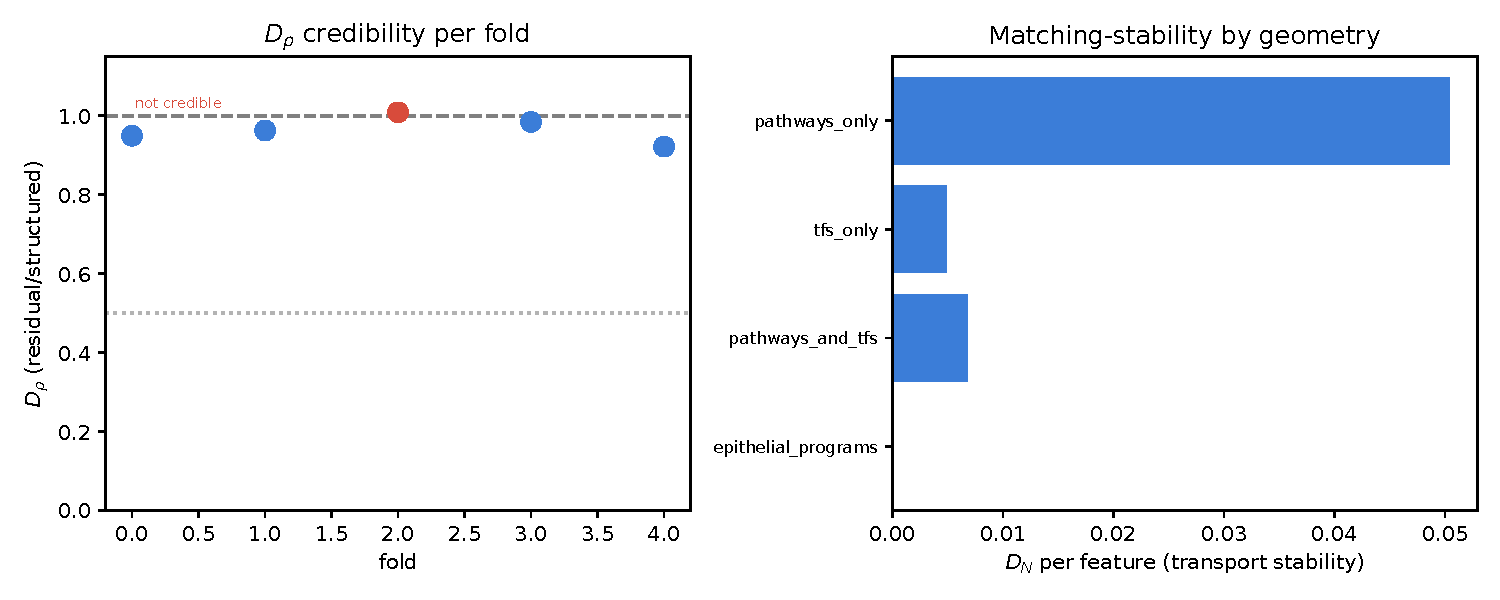
\includegraphics[width=0.92\textwidth]{figures/appendix/credibility_drho_transport.pdf}
  \caption[Decomposition credibility and transport-stability diagnostics]{Left: the credibility gate
  $D_\rho$ (residual-to-structured velocity ratio) per fold on the AAH$\rightarrow$AIS edge; four folds
  are credible ($D_\rho \leq 1$, blue) and fold 2 is marginally residual-dominated (red). Right: the
  normalized matching-stability diagnostic $D_N$ per feature by candidate regulatory geometry; the
  pathway sub-space is the most transport-stable block. Together these bound how much of the per-program
  $R_{\text{cond}}$ signal is attributable to the interpretable structured algebra versus the neural
  residuals.}
  \label{fig:app-c-credibility}
\end{figure}

Independent of the model, the regulatory feature space itself is stage-discriminative. A supervised
classifier of the $773$ self-features, trained and tested \emph{within} individual donors that
contribute both stages (so donor identity carries no information), separates the stages above chance in
every one of the eight donors shared across the Normal$\rightarrow$AAH edge (mean AUC $0.833$, SD
$0.103$; Figure~\ref{fig:app-c-within-donor}). This confirms that the geometry over which transport is
defined encodes the progression distinction; the below-chance cross-patient value reported in the main
text ($0.419$) therefore reflects a failure of cross-patient transfer, not an absence of stage signal.

\begin{figure}[htbp]
  \centering
  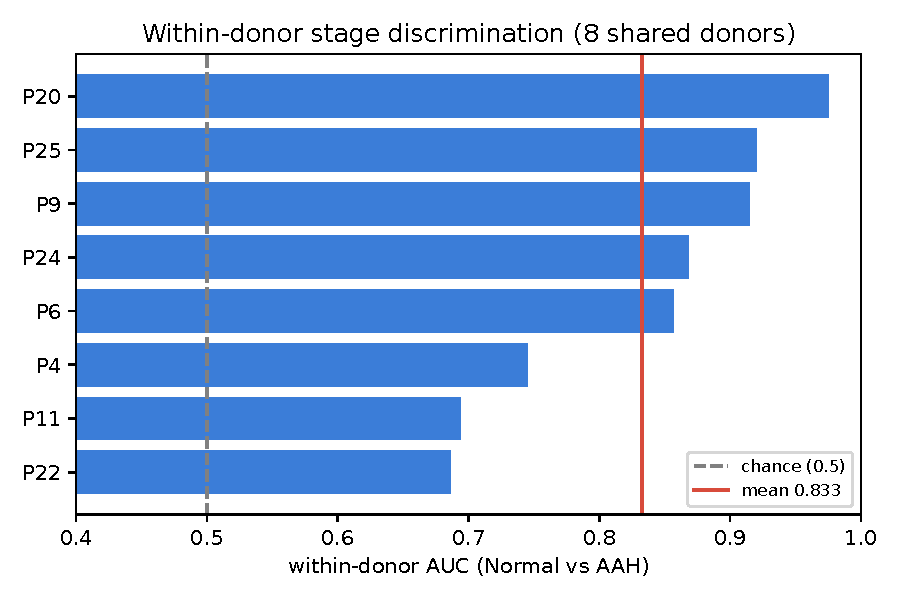
\includegraphics[width=0.7\textwidth]{figures/appendix/within_donor_auc_normal_aah.pdf}
  \caption[Within-donor stage discrimination]{Within-donor AUC for classifying Normal versus AAH from
  intrinsic regulatory self-features, for each of the eight donors that contribute both stages on the
  Normal$\rightarrow$AAH edge. Donor identity is held constant within each classification, so
  above-chance performance is stage biology rather than donor recognition. All eight donors exceed
  chance (mean $0.833$), demonstrating that the regulatory representation encodes stage independent of
  patient identity.}
  \label{fig:app-c-within-donor}
\end{figure}

\subsection{Training curves}\label{sec:app-c-training}

The three-stage training schedule converges cleanly on both LUAD edges: the Stage-A flow-matching
loss decays over its $1000$ steps, the Stage-B residual loss decays against the frozen-self target
over its $500$ steps, and the Stage-C anchored joint refinement produces only a small further
reduction, confirming that the identification set in Stages A and B is preserved rather than
overwritten. The per-stage convergence trace for each edge is shown in
Figure~\ref{fig:app-c-training}.



\begin{figure}[htbp]
  \centering
  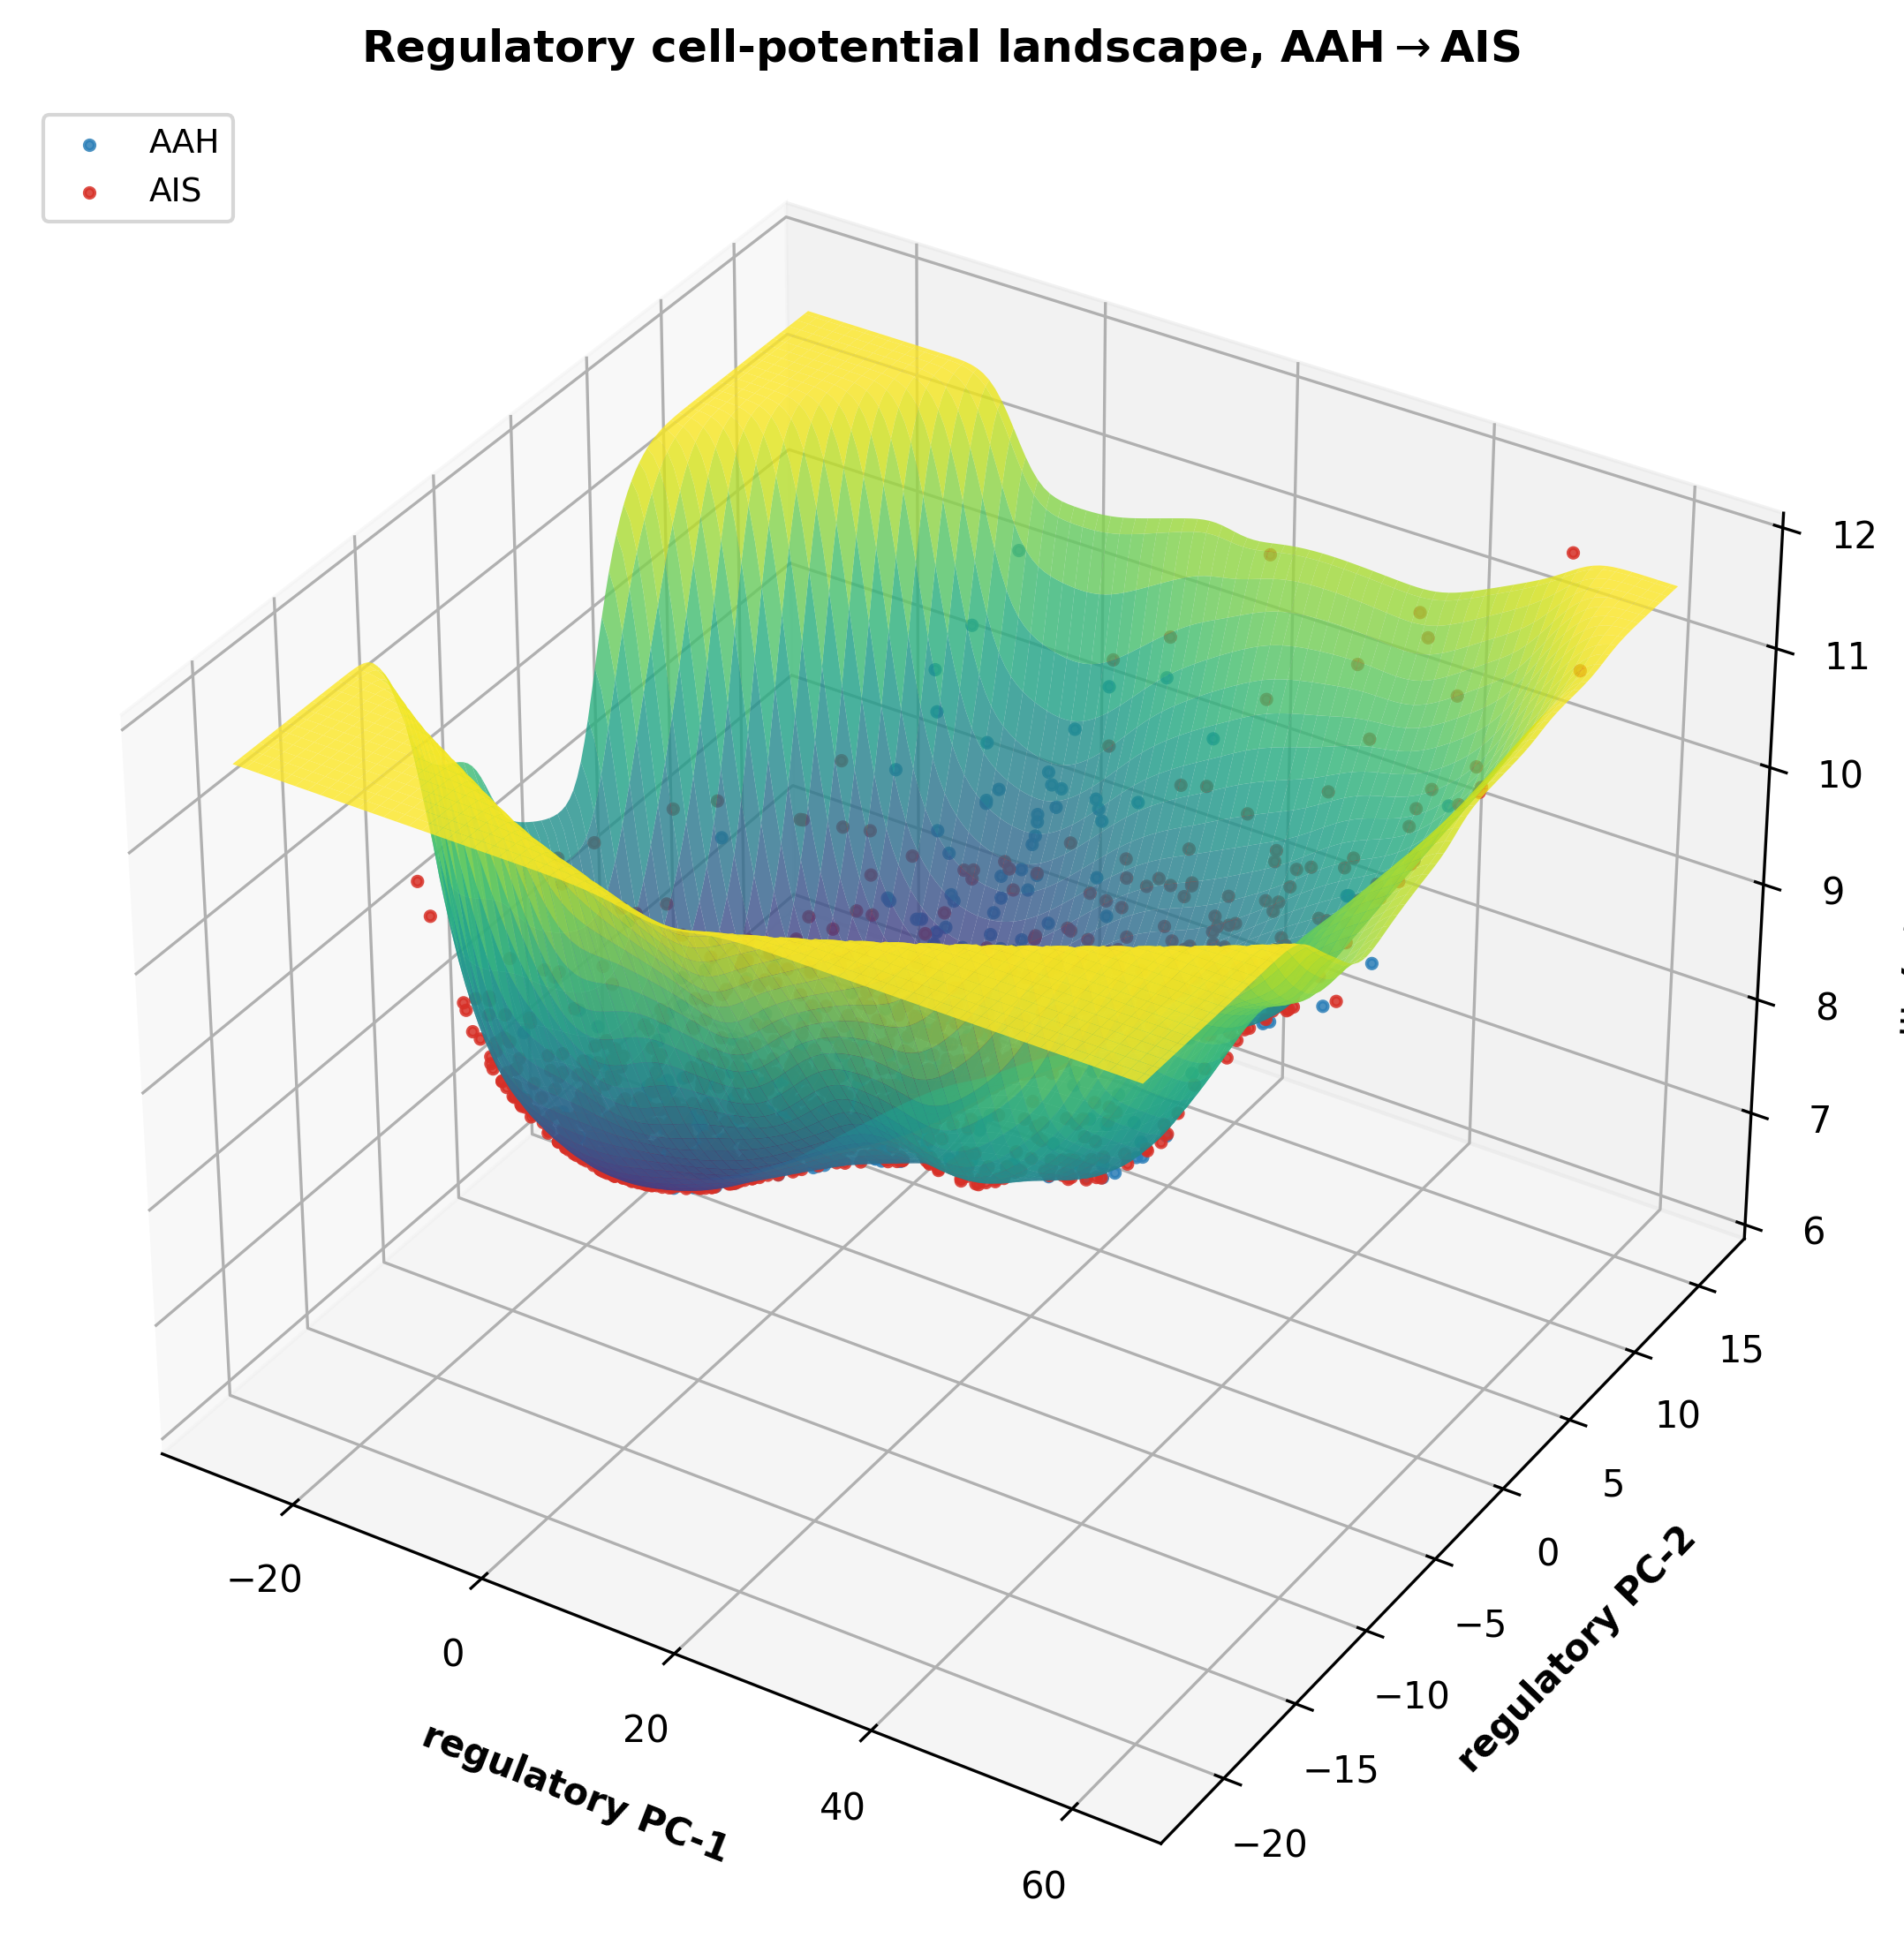
\includegraphics[width=0.8\textwidth]{figures/fig_waddington_landscape.png}
  \caption[Progression potential over the AAH and AIS epithelial clouds]{A $-\log$ density potential over the combined AAH and AIS epithelial clouds, with real integrated regulatory trajectories overlaid. The surface is an empirical $-\log$ density landscape, not a computed free energy; trajectories are integrated from the estimated regulatory transport operator.}
  \label{fig:waddington}
\end{figure}

% =====================================================================
\section{Complete falsification ladders}\label{sec:app-c-ladder}

The main text (Section~\ref{sec:results-ladder}) reports the load-bearing rungs of the falsification ladder.
Tables~\ref{tab:app-c-ladder-aah} and~\ref{tab:app-c-ladder-inv} give the complete per-fold semantic
Sinkhorn distances (lower is better) for every rung on the two LUAD edges, ordered by five-fold mean.
The full ladder adds the linear self-only and self-plus-context baselines
(\texttt{linear\_baseline\_A}, \texttt{linear\_baseline\_B}), the one-step non-integrated fields
(\texttt{one\_step\_full}, \texttt{one\_step\_structured\_C}), the monolithic MLP over concatenated
state/context/pseudo-time (\texttt{monolithic\_nn}), and the two degenerate grey-box variants
(\texttt{structured\_only} with the residual MLPs zeroed, \texttt{neural\_residuals\_only} with the
structured maps zeroed). Three further rungs (\texttt{spatial\_graph\_permutation},
\texttt{alt\_regulatory\_space}, \texttt{patient\_bootstrap\_replication}) are deferred and were not
scored under the common metric; they are omitted from the tables.

On AAH$\rightarrow$AIS the degenerate fields collapse as required (\texttt{structured\_only}
$2621.22$, \texttt{neural\_residuals\_only} $654.81$), \texttt{local\_context\_full} ($123.65$)
improves over \texttt{spatial\_self\_only} ($132.41$), and \texttt{local\_context\_full} does not
separate from \texttt{matched\_state\_shuffled} ($123.73$) or \texttt{donor\_stage\_average\_context}
($122.97$)---the ceiling reported in the main text. On AIS$\rightarrow$invasive
\texttt{local\_context\_full} ($265.59$) does not improve over \texttt{spatial\_self\_only}
($260.99$) and is essentially tied with \texttt{donor\_stage\_average\_context} ($259.72$) and its
own shuffle ($265.87$)---the invasion-edge refutation. The complete per-rung ladder for both edges is
shown in Figure~\ref{fig:app-c-ladder-bars}.

\begin{figure}[htbp]
  \centering
  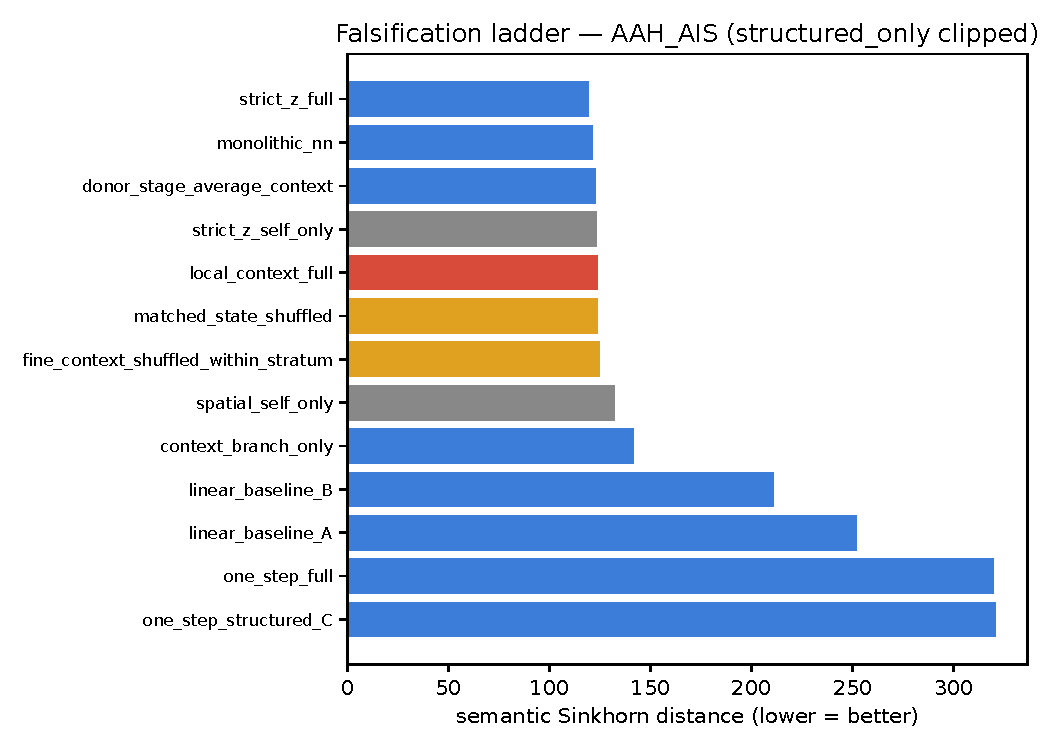
\includegraphics[width=0.49\textwidth]{figures/appendix/ladder_bar_AAH_AIS.pdf}\hfill
  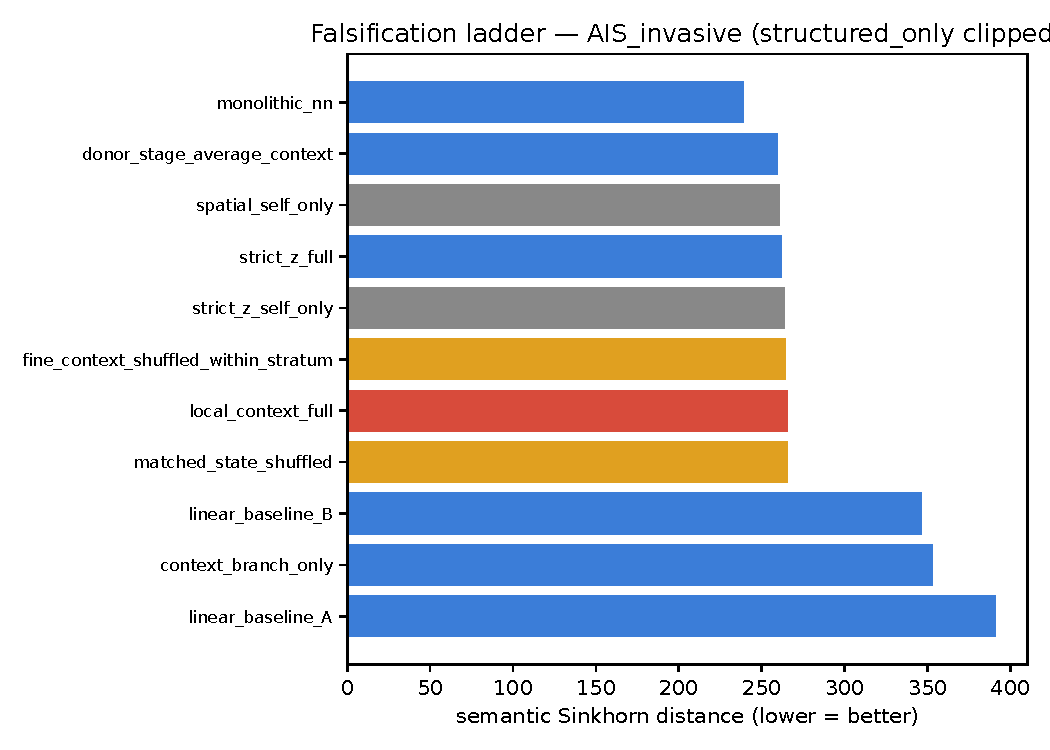
\includegraphics[width=0.49\textwidth]{figures/appendix/ladder_bar_AIS_invasive.pdf}
  \caption[Falsification-ladder bar charts, both LUAD edges]{Five-fold mean semantic Sinkhorn distance
  for every ladder rung (lower is better) on the AAH$\rightarrow$AIS edge (left) and the
  AIS$\rightarrow$invasive edge (right); the degenerate \texttt{structured\_only} rung is clipped so
  the informative range is visible. \texttt{local\_context\_full} (red) improves over
  \texttt{spatial\_self\_only} (grey) but does not separate from its stratum-matched shuffle (amber) or
  the specimen-level average, on both edges---the bounded reading reported in the main text.}
  \label{fig:app-c-ladder-bars}
\end{figure}

\begin{table}[htbp]
  \centering
  \caption[Complete AAH$\rightarrow$AIS falsification ladder]{Complete AAH$\rightarrow$AIS
  falsification ladder: per-fold and mean semantic Sinkhorn distance (lower is better), all rungs,
  ordered by mean.}
  \label{tab:app-c-ladder-aah}
  \footnotesize
  \begin{tabular}{lcccccc}
    \toprule
    Ladder rung & Fold 0 & Fold 1 & Fold 2 & Fold 3 & Fold 4 & Mean \\
    \midrule
    strict\_z\_full & 97.84 & 97.98 & 112.14 & 148.38 & 139.49 & 119.17 \\
    monolithic\_nn & 90.21 & 93.16 & 126.44 & 170.98 & 127.16 & 121.59 \\
    donor\_stage\_average\_context & 102.79 & 101.19 & 110.59 & 148.53 & 151.74 & 122.97 \\
    strict\_z\_self\_only & 101.03 & 101.06 & 117.50 & 153.03 & 143.02 & 123.13 \\
    local\_context\_full & 103.32 & 100.12 & 113.93 & 149.47 & 151.42 & 123.65 \\
    matched\_state\_shuffled & 103.40 & 101.21 & 112.61 & 150.29 & 151.15 & 123.73 \\
    fine\_context\_shuffled\_within\_stratum & 103.03 & 105.65 & 112.86 & 150.13 & 152.27 & 124.79 \\
    spatial\_self\_only & 109.14 & 122.16 & 128.19 & 152.20 & 150.36 & 132.41 \\
    context\_branch\_only & 121.26 & 116.34 & 153.68 & 177.74 & 139.52 & 141.71 \\
    linear\_baseline\_B & 162.80 & 249.26 & 128.14 & 191.28 & 322.65 & 210.83 \\
    linear\_baseline\_A & 156.27 & 190.16 & 334.42 & 290.62 & 287.85 & 251.86 \\
    one\_step\_full & 287.03 & 267.64 & 291.12 & 421.59 & 332.77 & 320.03 \\
    one\_step\_structured\_C & 289.77 & 268.88 & 291.47 & 419.67 & 333.36 & 320.63 \\
    neural\_residuals\_only & 654.55 & 693.56 & 571.26 & 805.72 & 548.93 & 654.81 \\
    structured\_only & 2435.72 & 2655.21 & 2822.41 & 3185.60 & 2007.17 & 2621.22 \\
    \bottomrule
  \end{tabular}
\end{table}

\begin{table}[htbp]
  \centering
  \caption[Complete AIS$\rightarrow$invasive falsification ladder]{Complete AIS$\rightarrow$invasive
  falsification ladder: per-fold and mean semantic Sinkhorn distance (lower is better), all rungs,
  ordered by mean.}
  \label{tab:app-c-ladder-inv}
  \footnotesize
  \begin{tabular}{lcccccc}
    \toprule
    Ladder rung & Fold 0 & Fold 1 & Fold 2 & Fold 3 & Fold 4 & Mean \\
    \midrule
    monolithic\_nn & 232.13 & 220.46 & 370.30 & 137.13 & 236.09 & 239.22 \\
    donor\_stage\_average\_context & 236.45 & 270.00 & 355.06 & 154.28 & 282.83 & 259.72 \\
    spatial\_self\_only & 238.40 & 273.87 & 359.59 & 159.32 & 273.76 & 260.99 \\
    strict\_z\_full & 230.98 & 293.97 & 367.84 & 139.02 & 276.71 & 261.71 \\
    strict\_z\_self\_only & 235.50 & 282.52 & 371.62 & 140.27 & 288.36 & 263.66 \\
    fine\_context\_shuffled\_within\_stratum & 235.63 & 281.63 & 355.54 & 164.18 & 283.67 & 264.13 \\
    local\_context\_full & 241.33 & 284.45 & 355.40 & 160.20 & 286.54 & 265.59 \\
    matched\_state\_shuffled & 235.14 & 286.39 & 358.19 & 166.27 & 283.35 & 265.87 \\
    linear\_baseline\_B & 322.01 & 370.45 & 492.23 & 234.70 & 313.05 & 346.49 \\
    context\_branch\_only & 295.16 & 354.67 & 476.07 & 188.91 & 450.08 & 352.98 \\
    linear\_baseline\_A & 450.79 & 367.96 & 508.37 & 283.33 & 343.53 & 390.80 \\
    one\_step\_full & 356.79 & 509.33 & 489.46 & 341.68 & 633.70 & 466.19 \\
    one\_step\_structured\_C & 357.34 & 509.78 & 489.08 & 341.38 & 633.41 & 466.20 \\
    neural\_residuals\_only & 913.42 & 912.21 & 858.28 & 794.37 & 747.29 & 845.11 \\
    structured\_only & 3041.00 & 2271.35 & 2993.02 & 2514.49 & 2725.79 & 2709.13 \\
    \bottomrule
  \end{tabular}
\end{table}

% =====================================================================
\section{Program-stability atlas}\label{sec:app-c-stability}

Per-program conditional transport $R_{\mathrm{cond}}$ was estimated for all $773$ programs on each
LUAD edge across the five patient-held-out folds. A program is classed STABLE only when its held-out
confidence interval excludes zero and holds sign in every fold, DIRECTIONALLY\_STABLE when the
interval excludes zero on aggregate, and UNSTABLE otherwise. On AAH$\rightarrow$AIS the classification
is $29$ STABLE, $30$ DIRECTIONALLY\_STABLE, and $714$ UNSTABLE; on AIS$\rightarrow$invasive it is
$28$ STABLE, $38$ DIRECTIONALLY\_STABLE, and $707$ UNSTABLE. The complete $773$-program tables (mean
$R_{\mathrm{cond}}$, confidence bounds, fold standard deviation, sign consistency, and class) are
provided as machine-readable files (\texttt{Re\_per\_program\_<edge>\_v2lowrank\_source.parquet};
dossier CSVs \texttt{Rcond\_ALL\_AAH\_AIS.csv} and \texttt{Rcond\_ALL\_AIS\_invasive.csv}).
Table~\ref{tab:app-c-stable-aah} lists the $29$ STABLE programs of the AAH$\rightarrow$AIS edge in
full, with mean $R_{\mathrm{cond}}$ and its held-out $95\%$ confidence interval. The full
$R_{\mathrm{cond}}$ spectrum across all $773$ programs is shown in Figure~\ref{fig:app-c-spectrum}.

\begin{figure}[htbp]
  \centering
  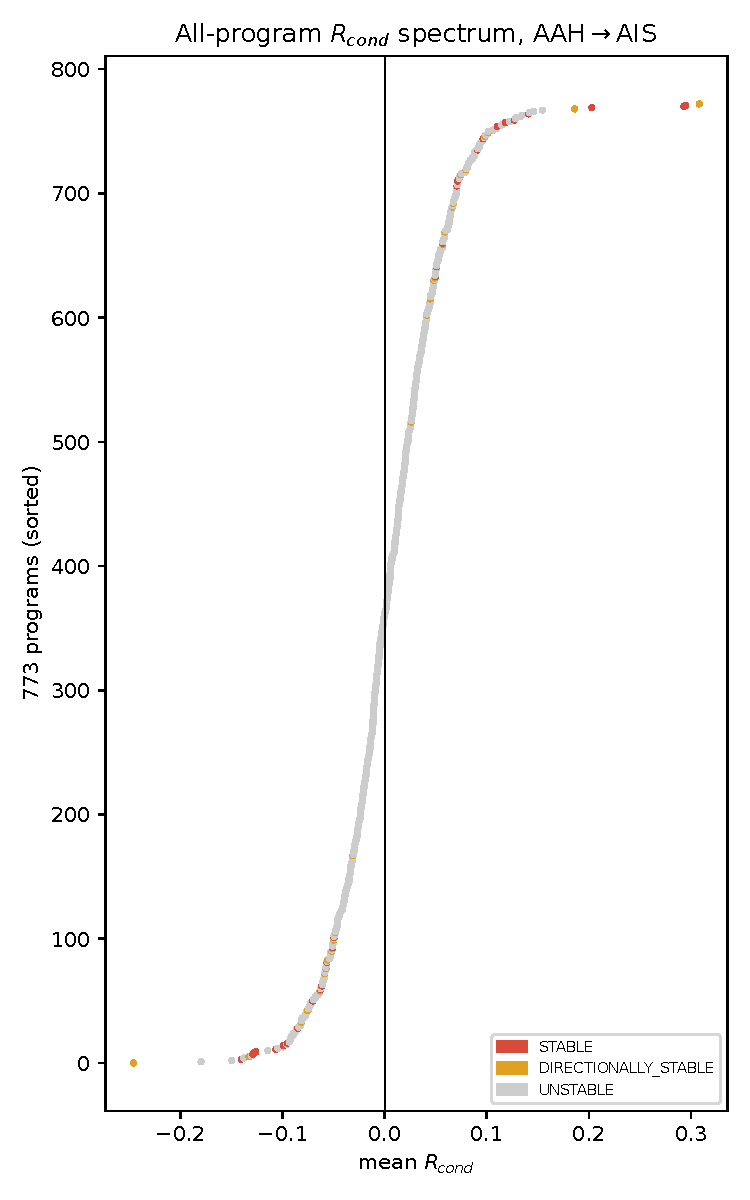
\includegraphics[width=0.6\textwidth]{figures/appendix/all_program_spectrum_AAH_AIS.pdf}
  \caption[All-program $R_{\mathrm{cond}}$ spectrum, AAH$\rightarrow$AIS]{Mean conditional transport
  $R_{\mathrm{cond}}$ for all $773$ regulatory programs on the AAH$\rightarrow$AIS edge, sorted by
  effect and colored by cross-fold stability class. The STABLE (red) and DIRECTIONALLY\_STABLE (amber)
  programs occupy the tails; the large UNSTABLE majority (grey) clusters near zero, which is the
  expected shape for a conditional effect that must survive patient-level resampling.}
  \label{fig:app-c-spectrum}
\end{figure}

\begin{longtable}{lccc}
  \caption[STABLE programs, AAH$\rightarrow$AIS]{The $29$ STABLE regulatory programs on the
  AAH$\rightarrow$AIS edge, with mean conditional transport $R_{\mathrm{cond}}$ and held-out $95\%$
  confidence interval, ordered from most context-upregulated to most context-downregulated.}
  \label{tab:app-c-stable-aah} \\
  \toprule
  Program & $R_{\mathrm{cond}}$ & CI lower & CI upper \\
  \midrule
  \endfirsthead
  \toprule
  Program & $R_{\mathrm{cond}}$ & CI lower & CI upper \\
  \midrule
  \endhead
  \midrule \multicolumn{4}{r}{\emph{continued on next page}} \\
  \endfoot
  \bottomrule
  \endlastfoot
  pathway\_p53 & $+0.295$ & $+0.246$ & $+0.344$ \\
  pathway\_WNT & $+0.293$ & $+0.255$ & $+0.331$ \\
  pathway\_Trail & $+0.203$ & $+0.184$ & $+0.221$ \\
  tf\_FOS & $+0.141$ & $+0.124$ & $+0.157$ \\
  tf\_KAT5 & $+0.127$ & $+0.114$ & $+0.140$ \\
  tf\_PAX8 & $+0.118$ & $+0.105$ & $+0.131$ \\
  tf\_RB1 & $+0.110$ & $+0.094$ & $+0.127$ \\
  tf\_ETV5 & $+0.096$ & $+0.077$ & $+0.115$ \\
  tf\_NCOR2 & $+0.091$ & $+0.073$ & $+0.108$ \\
  tf\_HESX1 & $+0.072$ & $+0.060$ & $+0.084$ \\
  tf\_SPIC & $+0.071$ & $+0.056$ & $+0.086$ \\
  tf\_YBX3 & $+0.071$ & $+0.056$ & $+0.086$ \\
  tf\_ELF2 & $+0.057$ & $+0.047$ & $+0.066$ \\
  tf\_DOT1L & $+0.051$ & $+0.031$ & $+0.070$ \\
  tf\_FHL2 & $+0.049$ & $+0.036$ & $+0.063$ \\
  tf\_ZNF219 & $-0.050$ & $-0.058$ & $-0.041$ \\
  tf\_PPARGC1B & $-0.051$ & $-0.057$ & $-0.046$ \\
  tf\_PITX1 & $-0.057$ & $-0.073$ & $-0.040$ \\
  tf\_ZNF382 & $-0.061$ & $-0.075$ & $-0.048$ \\
  tf\_ARX & $-0.063$ & $-0.071$ & $-0.055$ \\
  tf\_MYT1 & $-0.071$ & $-0.080$ & $-0.061$ \\
  tf\_SATB1 & $-0.085$ & $-0.103$ & $-0.068$ \\
  tf\_NFE2L3 & $-0.095$ & $-0.105$ & $-0.085$ \\
  tf\_SMAD4 & $-0.099$ & $-0.110$ & $-0.088$ \\
  tf\_ETV6 & $-0.106$ & $-0.134$ & $-0.079$ \\
  tf\_ETV3 & $-0.126$ & $-0.131$ & $-0.121$ \\
  tf\_IRF9 & $-0.129$ & $-0.154$ & $-0.103$ \\
  tf\_GLI3 & $-0.129$ & $-0.134$ & $-0.124$ \\
  tf\_ZBTB18 & $-0.140$ & $-0.167$ & $-0.114$ \\
\end{longtable}


\begin{figure}[htbp]
  \centering
  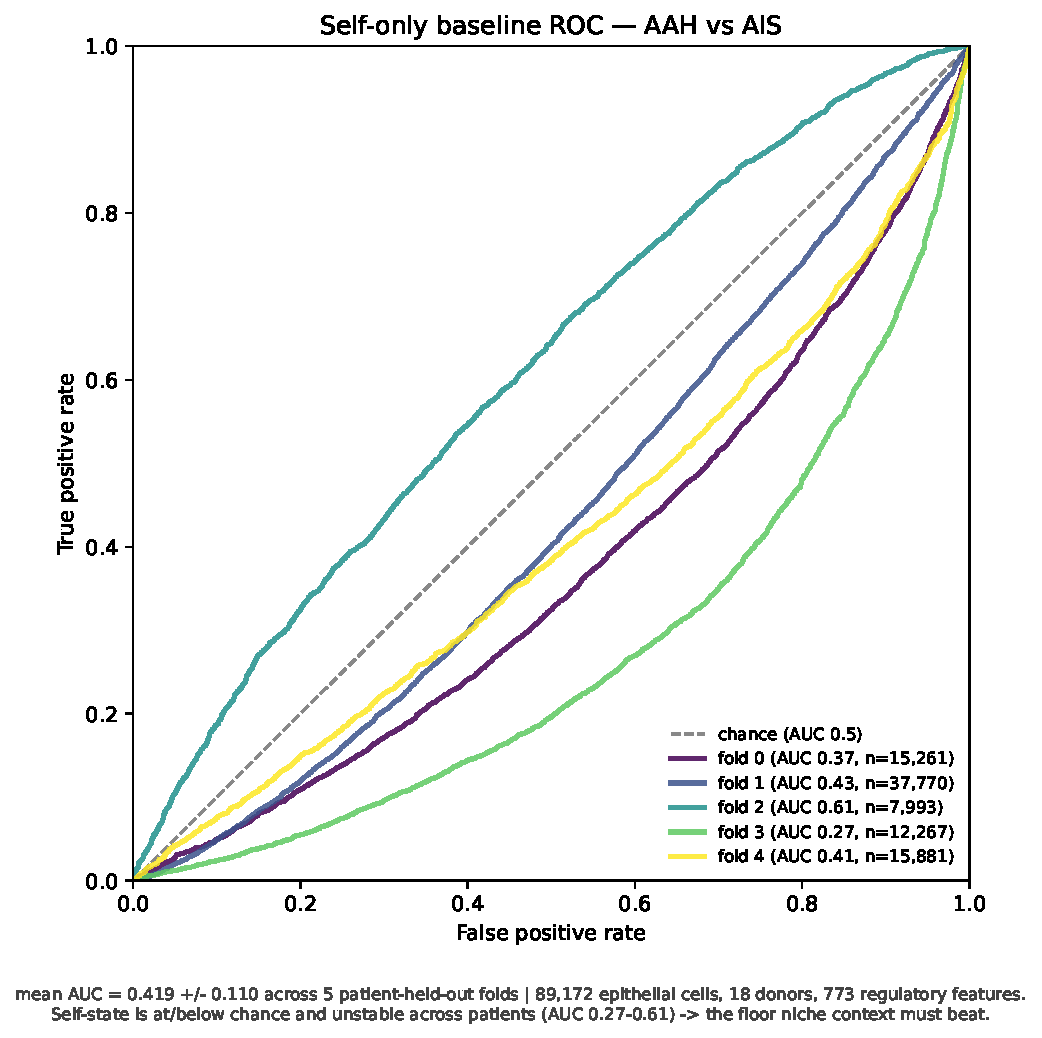
\includegraphics[width=0.75\textwidth]{figures/ude_result/self_only_AAH_AIS_roc.pdf}
  \caption[Self-only baseline ROC, AAH vs AIS]{Per-fold receiver-operating-characteristic curves for a self-only classifier of AAH versus AIS on intrinsic epithelial regulatory state, under \emph{donor}-held-out cross-validation (mean AUC $0.419 \pm 0.110$; per-fold $0.27$--$0.61$; 89{,}172 epithelial cells, 18 donors, 773 regulatory features). The mean is approximately $1.6$ standard errors below $0.5$, i.e.\ at chance out of sample, indicating that intrinsic regulatory state does not transfer across patients; see the text for the pooled and within-donor comparisons that localize this to a donor-entangled representation. This cross-patient instability motivates the patient-held-out evaluation used throughout.}
  \label{fig:self-only-roc}
\end{figure}

% =====================================================================
\section{Spatial niche-association}\label{sec:app-c-niche}

To test whether regulatory redirection concentrates in a specific ecological context, the per-receiver
signed $R_{\mathrm{cond}}$ was averaged, donor-adjusted, within each of the three niche strata
identified by the coarse stratifier (stratum~0 to stratum~2, ordered by increasing CAF/immune
density). Table~\ref{tab:app-c-niche} reports the leading stable programs across strata for both
LUAD edges. The programs move monotonically but modestly with stratum: on AAH$\rightarrow$AIS,
JAK-STAT deepens from $-0.191$ to $-0.308$, WNT rises from $+0.275$ to $+0.311$, and p53 declines
from $+0.363$ to $+0.240$; the same ordering (JAK-STAT $-0.171 \rightarrow -0.303$) holds on
AIS$\rightarrow$invasive. The direction is consistent with an inflammatory-ecology reading, but the
across-stratum magnitude is small relative to each program's overall effect, supporting the main-text
conclusion that redirection is graded by coarse ecological stratum rather than switched by a single
niche identity. These values are computed on the per-receiver $R_{\mathrm{cond}}$ tables
($10$ AAH$\rightarrow$AIS donors, $12$ AIS$\rightarrow$invasive donors) and are authoritative.

\begin{table}[htbp]
  \centering
  \caption[Per-stratum conditional transport for leading programs]{Donor-adjusted mean
  $R_{\mathrm{cond}}$ for the leading stable programs across the three niche strata (stratum~0 low to
  stratum~2 high CAF/immune density), both LUAD edges. Monotonic but modest gradients.}
  \label{tab:app-c-niche}
  \footnotesize
  \begin{tabular}{llccc}
    \toprule
    Edge & Program & Stratum 0 & Stratum 1 & Stratum 2 \\
    \midrule
    AAH$\rightarrow$AIS      & JAK-STAT & $-0.191$ & $-0.258$ & $-0.308$ \\
                             & WNT      & $+0.275$ & $+0.288$ & $+0.311$ \\
                             & Trail    & $+0.182$ & $+0.196$ & $+0.220$ \\
                             & p53      & $+0.363$ & $+0.294$ & $+0.240$ \\
    \midrule
    AIS$\rightarrow$invasive & JAK-STAT & $-0.171$ & $-0.261$ & $-0.303$ \\
                             & WNT      & $+0.296$ & $+0.275$ & $+0.262$ \\
                             & Trail    & $+0.260$ & $+0.278$ & $+0.283$ \\
    \bottomrule
  \end{tabular}
\end{table}

\subsection{Descriptive tissue ecology across the preinvasive edge}
\label{sec:app-c-ecology}

Table~\ref{tab:app-c-ecology} reports the donor-level mean abundance of the major ecological
compartments in AAH versus AIS, computed on the authoritative full-cohort spatial-context table
(\texttt{w\_AAH\_AIS.parquet}; 10 AAH and 12 AIS donors). No compartment differs at a donor-level
Benjamini--Hochberg $q<0.05$ (minimum $q=0.79$): the marginal composition of these ecological
compartments does not separate AAH from AIS at the donor level in the full cohort. This is consistent
with the variance decomposition (Section~\ref{sec:app-c-niche}), in which between-stage variance in
these features is under $1\%$; the informative ecological signal is not in the stage-level marginal
composition. Malignant fraction shows the largest (still non-significant) directional increase toward
AIS ($+0.015$), and alveolar-macrophage abundance the largest directional decrease ($-0.007$).

\begin{table}[htbp]
  \centering
  \caption[Tissue-ecology composition, AAH vs AIS]{Donor-level mean compartment abundance in AAH vs
  AIS on the authoritative full-cohort spatial-context table (10 AAH / 12 AIS donors; Welch $t$ per
  compartment). No compartment clears a Benjamini--Hochberg $q<0.05$ (min $q=0.79$): stage-level
  marginal composition does not separate the two stages at the donor level.}
  \label{tab:app-c-ecology}
  \footnotesize
  \begin{tabular}{lcccc}
    \toprule
    Compartment & Mean AAH & Mean AIS & $\Delta$(AIS$-$AAH) & $p$ \\
    \midrule
    Alveolar macrophage & $0.063$ & $0.057$ & $-0.007$ & $0.646$ \\
    Macrophage (total)  & $0.026$ & $0.026$ & $+0.000$ & $0.995$ \\
    Fibroblast          & $0.111$ & $0.102$ & $-0.009$ & $0.388$ \\
    CAF fraction        & $0.116$ & $0.107$ & $-0.009$ & $0.423$ \\
    Immune fraction     & $0.238$ & $0.226$ & $-0.012$ & $0.661$ \\
    Malignant fraction  & $0.023$ & $0.038$ & $+0.015$ & $0.185$ \\
    \bottomrule
  \end{tabular}
\end{table}

\subsection{Macrophage niche and context-residual transport}
\label{sec:app-c-macrophage}

A pre-registered hypothesis of this work is that an inflammatory macrophage niche is associated with
the context-driven regulatory programs. Table~\ref{tab:app-c-il1b} reports a mixed model of
per-receiver $R_{\mathrm{cond}}$ on macrophage abundance (donor random intercept) on the authoritative
full-cohort spatial-context table (66{,}834 receivers across 10 donors). The association holds and is
directionally coherent: the inflammatory and stress programs JAK-STAT ($+0.043$ per SD macrophage),
NF$\kappa$B ($+0.039$), p53 ($+0.038$), and EGFR ($+0.041$) all increase their context effect with
local macrophage density, while Hypoxia decreases weakly ($-0.015$). Because this association survives
on the full cohort, the JAK-STAT/NF$\kappa$B arm is reported in the main-text Results
(Section~\ref{sec:comm} context) as the macrophage-associated inflammatory signature; the remaining
programs are tabulated here. One caveat qualifies the confidence intervals: with per-spot observations
the donor random-effect variance is near-singular, so the intervals are narrower than a fully
donor-level test would give---the \emph{direction and rank} of the association are the robust readout,
not the exact interval width.

\begin{table}[htbp]
  \centering
  \caption[Macrophage niche vs context residual, AAH$\rightarrow$AIS]{Mixed-model slope of
  per-receiver $R_{\mathrm{cond}}$ on total-macrophage abundance (per SD, donor random intercept) on
  the authoritative full-cohort spatial-context table (66{,}834 receivers, 10 donors). Inflammatory and
  stress programs increase their context effect with macrophage density. Intervals are model-based;
  per-spot sampling makes the donor variance near-singular, so direction and rank are the robust
  readout.}
  \label{tab:app-c-il1b}
  \footnotesize
  \begin{tabular}{lcc}
    \toprule
    Program & $\beta$ per SD macrophage & 95\% CI \\
    \midrule
    JAK-STAT & $+0.043$ & $[+0.040,\,+0.046]$ \\
    NF$\kappa$B  & $+0.039$ & $[+0.035,\,+0.042]$ \\
    EGFR     & $+0.041$ & $[+0.037,\,+0.045]$ \\
    p53      & $+0.038$ & $[+0.036,\,+0.040]$ \\
    Hypoxia  & $-0.015$ & $[-0.017,\,-0.012]$ \\
    \bottomrule
  \end{tabular}
\end{table}

\subsection{R\textsubscript{cond}-gated cell--cell communication}
\label{sec:app-c-comm}

Section~\ref{sec:comm} defines the R\textsubscript{cond}-gated communication framework
and reports its headline result; the complete full-cohort output is given here. The framework infers
ligand-receptor interactions by LIANA consensus per stage, wires receptor$\rightarrow$TF edges from
OmniPath, retains only chains whose terminal TF program is \textsc{stable} or
\textsc{directionally stable}
with $|R_{\mathrm{cond}}|\geq0.05$, and scores each retained chain by the product of its L--R strength
and the terminal program's context effect. Table~\ref{tab:app-c-comm-chains} lists the top gated chains
per LUAD edge; all numbers derive from the completed full-cohort run
(\texttt{outputs/comm/\{AAH\_AIS,AIS\_invasive\}/gated\_chains\_all.csv}).

\begin{table}[htbp]
  \centering
  \caption[Top R\textsubscript{cond}-gated communication chains]{Top $R_{\mathrm{cond}}$-gated
  sender$\rightarrow$ligand$\rightarrow$receptor$\rightarrow$program chains per LUAD edge, ranked by
  chain score (product of L--R strength and terminal-program $|R_{\mathrm{cond}}|$). All terminal
  programs are stable (STA) or directionally-stable (DIR) context-driven programs from the per-program
  analysis.}
  \label{tab:app-c-comm-chains}
  \footnotesize
  \begin{tabular}{llllrcr}
    \toprule
    Sender & Ligand & Receptor & Program & $R_{\mathrm{cond}}$ & Class & Score \\
    \midrule
    \multicolumn{7}{l}{\emph{AAH$\rightarrow$AIS}} \\
    SMG\_Serous & LTF & IL1RL1 & RB1 & $+0.110$ & STA & 0.368 \\
    Mesothelia & C3 & LRP1 & RB1 & $+0.110$ & STA & 0.358 \\
    Macro\_CHIT1 & APOE & LRP1 & RB1 & $+0.110$ & STA & 0.351 \\
    Mesothelia & PLA2G2A & EGFR & FOS & $+0.141$ & STA & 0.320 \\
    Macro\_alveolar & GRN & EGFR & FOS & $+0.141$ & STA & 0.314 \\
    Fibro\_alveolar & A2M & LRP1 & RB1 & $+0.110$ & STA & 0.312 \\
    \midrule
    \multicolumn{7}{l}{\emph{AIS$\rightarrow$invasive}} \\
    Mesothelia & PLA2G2A & EGFR & HDAC1 & $-0.204$ & DIR & 0.463 \\
    Macro\_alveolar & GRN & EGFR & HDAC1 & $-0.204$ & DIR & 0.454 \\
    Macro\_CHIT1 & PSAP & AR & HSF2 & $+0.225$ & DIR & 0.424 \\
    NAF\_perineurial & DCN & EGFR & HDAC1 & $-0.204$ & DIR & 0.411 \\
    Fibro\_alveolar & DCN & EGFR & HDAC1 & $-0.204$ & DIR & 0.397 \\
    \bottomrule
  \end{tabular}
\end{table}

At the tissue scale, the differential communication network (AIS versus AAH) reorganizes around a
small number of sender hubs. Mesothelial, submucosal-gland-basal, and dividing-basal populations gain
the most net signaling into the epithelial and stromal compartment at AIS, while a perineurial-fibroblast
and myoepithelial band loses signaling (Figure~\ref{fig:app-c-comm-heatmap}); the same reorganization is
shown as a differential chord diagram in Figure~\ref{fig:app-c-comm-circos}. These tissue-wide views are
descriptive summaries of the LIANA differential network and are not $R_{\mathrm{cond}}$-gated; the gated
chains above are the subset that terminate on model-identified context-driven programs.

\begin{figure}[htbp]
  \centering
  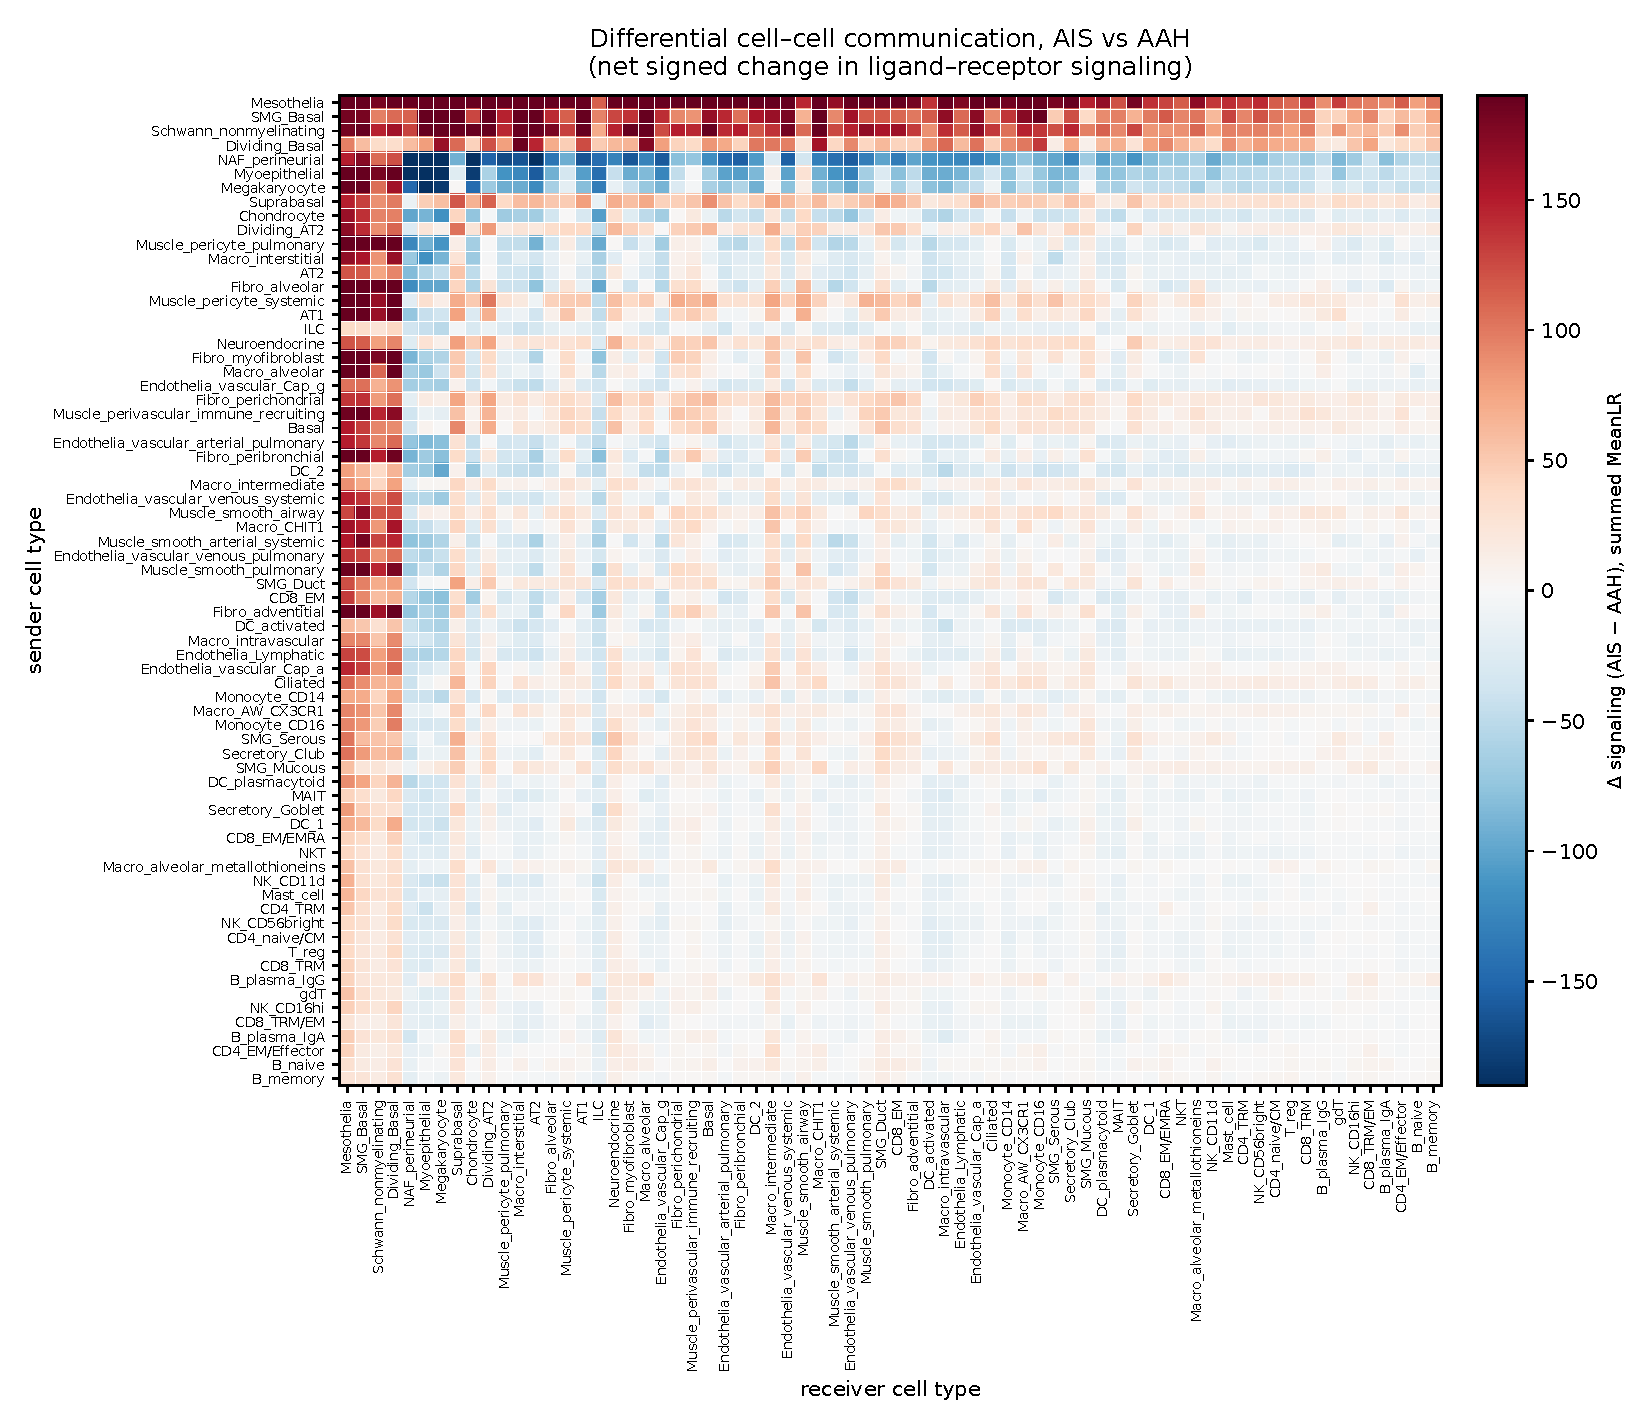
\includegraphics[width=0.92\textwidth]{figures/comm/differential_cci_heatmap_AAH_AIS.pdf}
  \caption[Differential cell--cell communication heatmap, AAH$\rightarrow$AIS]{Net signed change in
  ligand--receptor signaling between AIS and AAH for every sender$\times$receiver cell-type pair (summed
  over all L--R pairs; red gained at AIS, blue lost), ordered by total absolute activity. Mesothelial,
  submucosal-gland, and dividing-basal senders gain signaling broadly across the tissue; a
  perineurial/myoepithelial band loses it.}
  \label{fig:app-c-comm-heatmap}
\end{figure}

\begin{figure}[htbp]
  \centering
  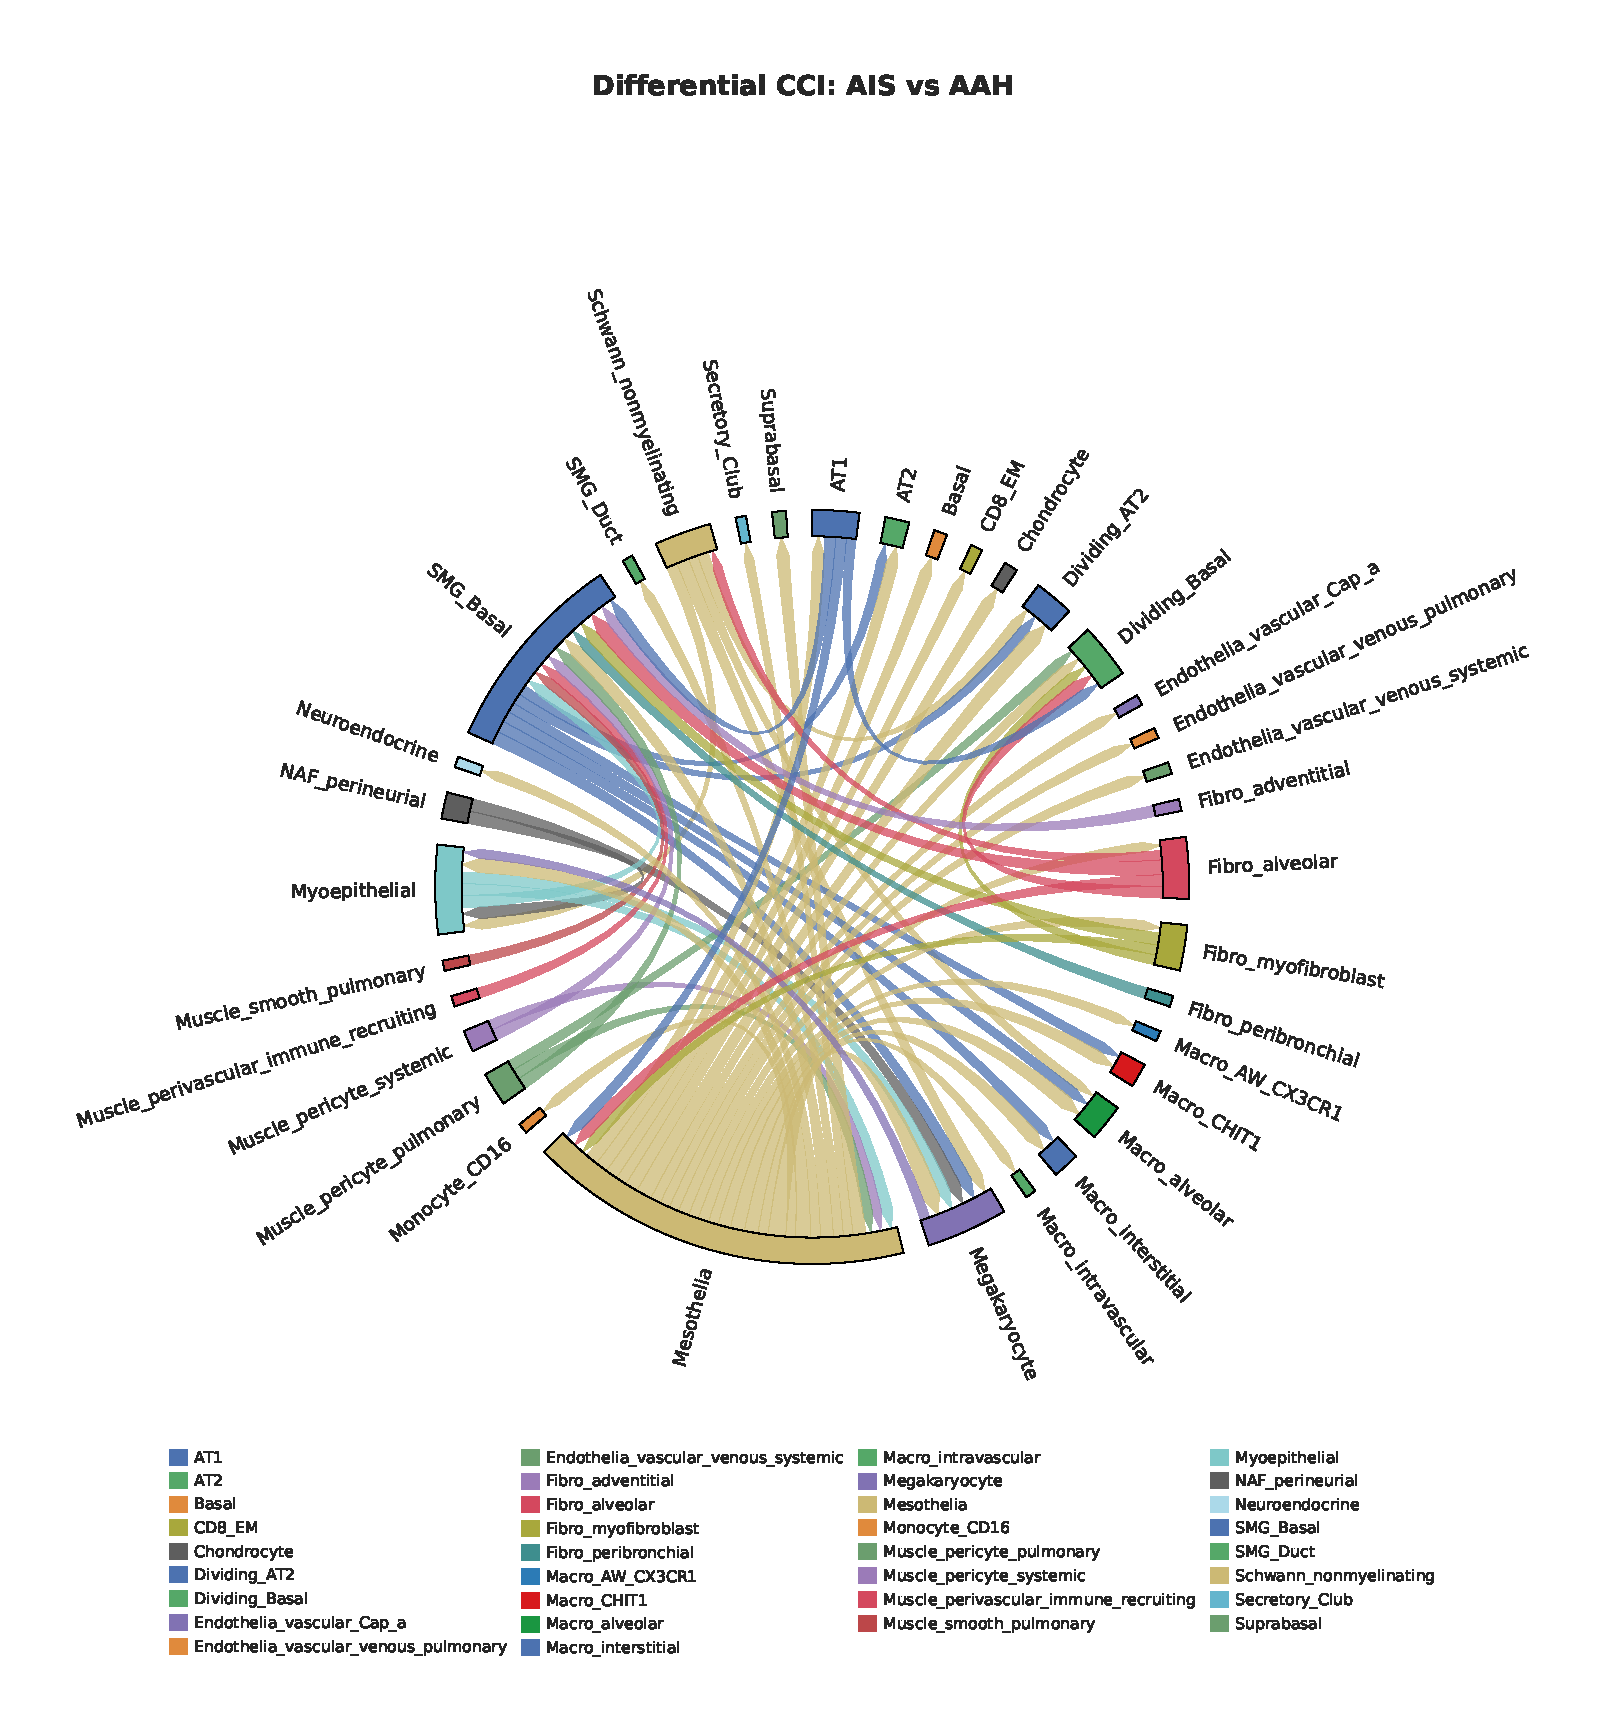
\includegraphics[width=0.8\textwidth]{figures/comm/circos_differential_AAH_AIS.pdf}
  \caption[Differential communication chord diagram, AAH$\rightarrow$AIS]{Differential cell--cell
  interaction network (AIS versus AAH) as a chord diagram; ribbon width encodes the net change in
  signaling between each cell-type pair. The same reorganization as Figure~\ref{fig:app-c-comm-heatmap},
  emphasizing the dominant sender hubs.}
  \label{fig:app-c-comm-circos}
\end{figure}


\begin{figure}[htbp]
  \centering
  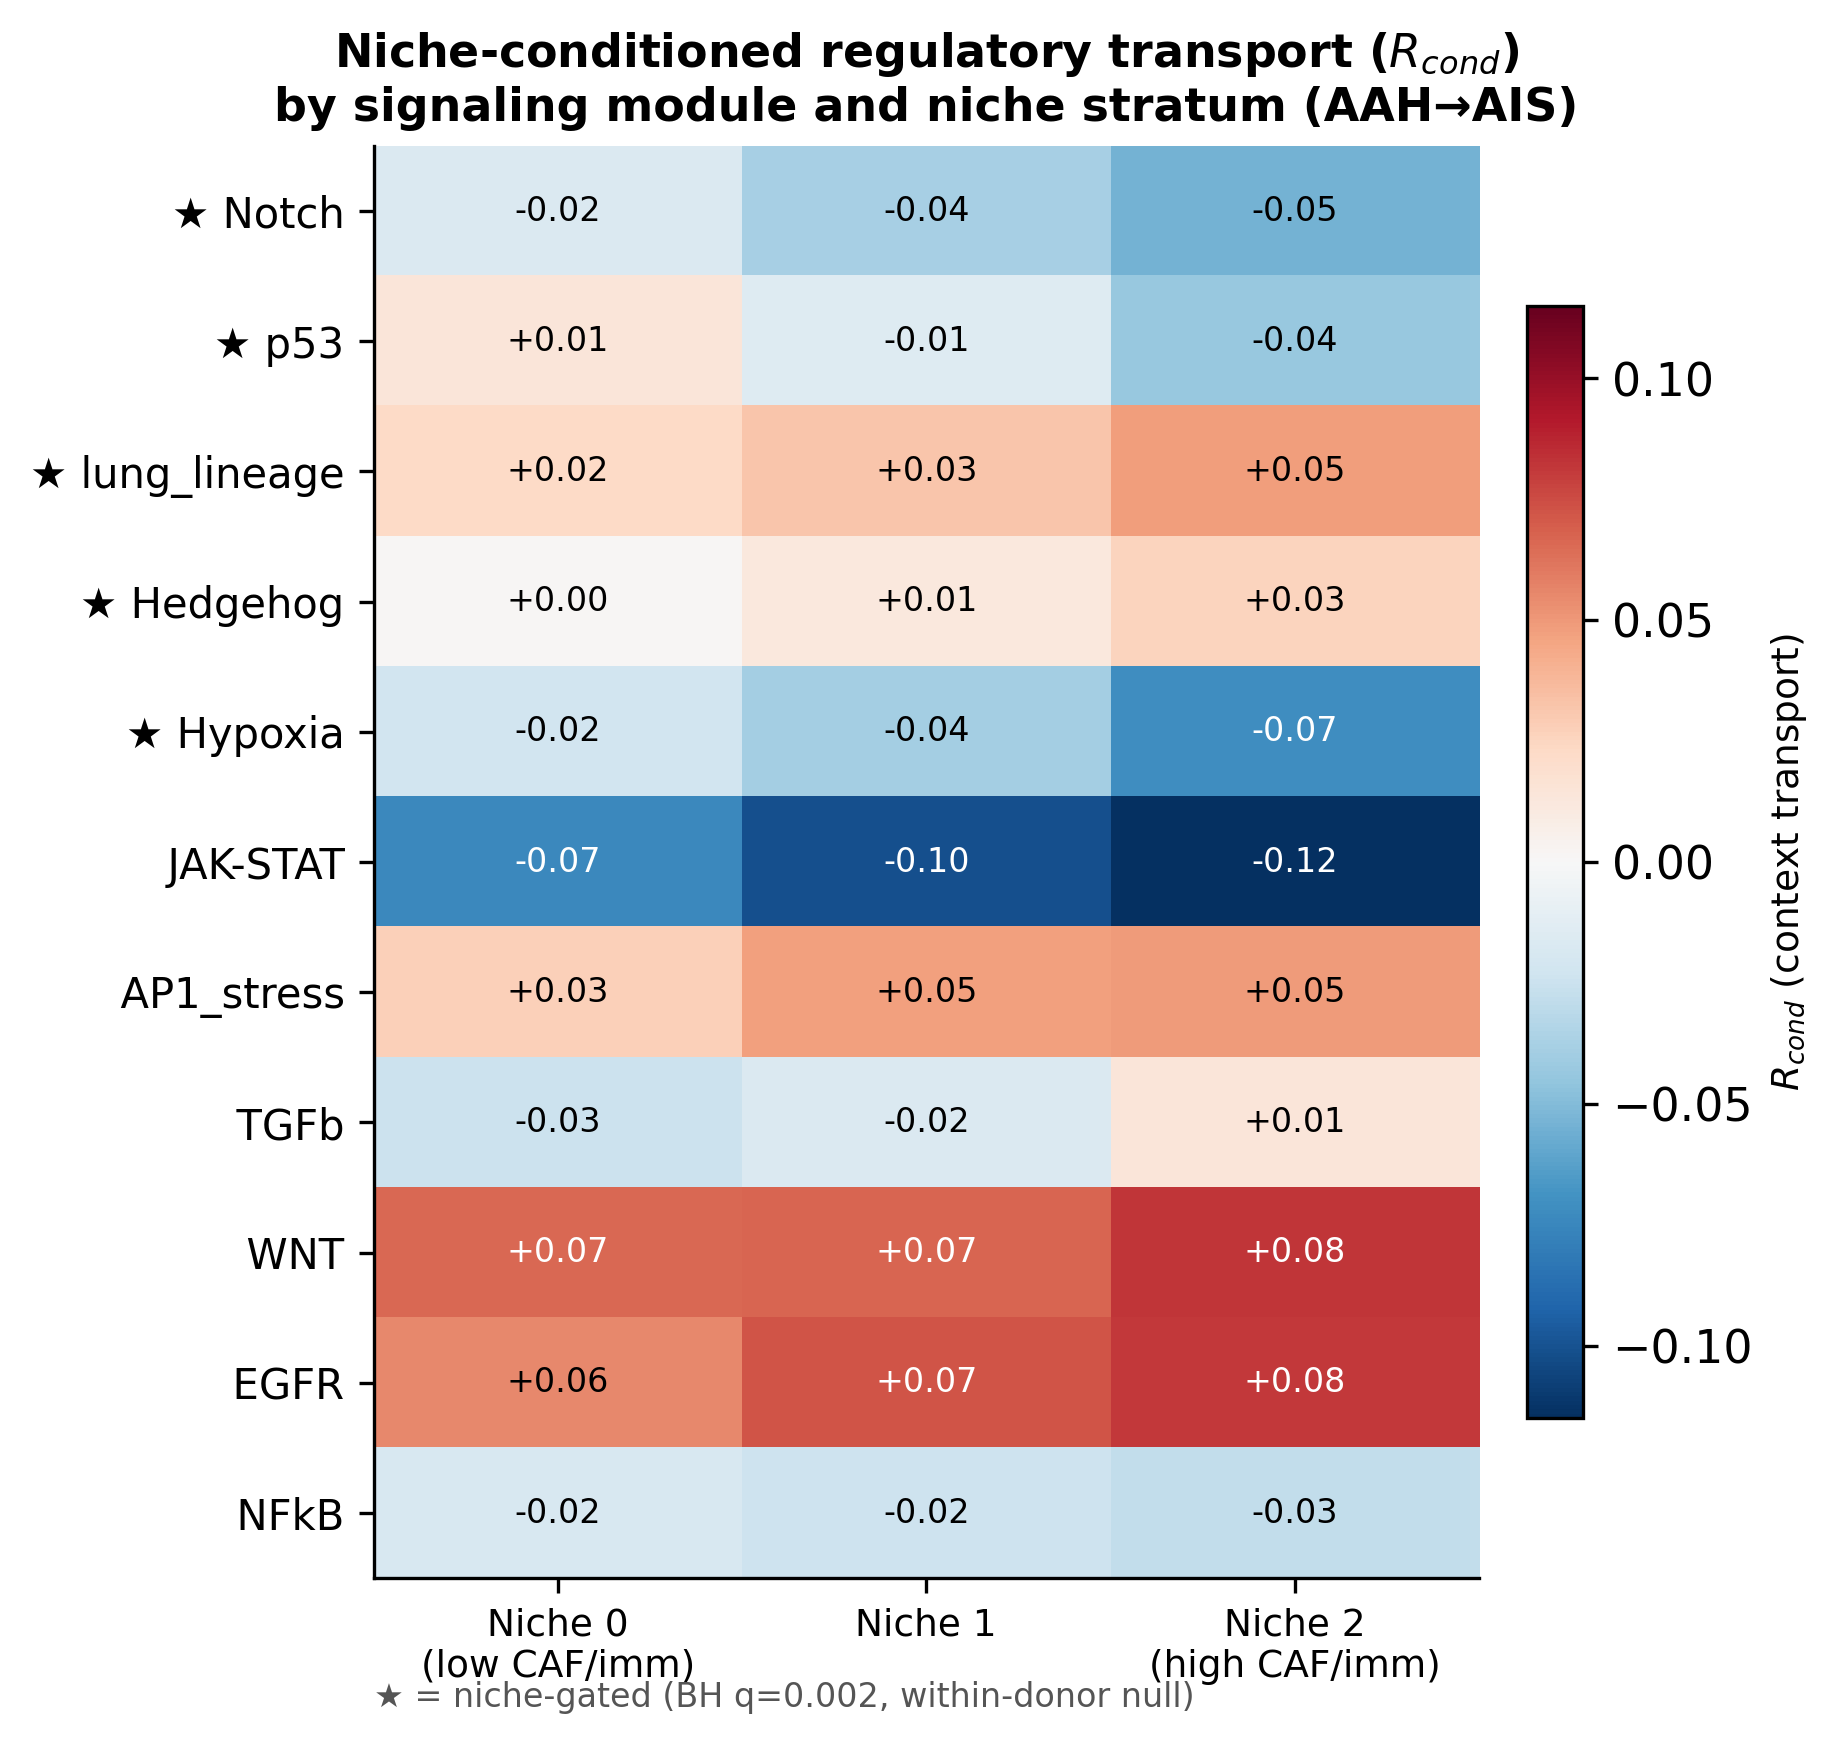
\includegraphics[width=0.85\textwidth]{figures/fig_niche_module_heatmap.png}
  \caption[Niche $\times$ regulatory-module conditional transport]{Conditional transport $R_{\text{cond}}$ for curated regulatory modules across the three niche strata (ordered from low to high CAF/immune density). Modules move only weakly across strata relative to a within-donor permutation null, consistent with the coarse-ecology reading: regulatory redirection tracks the stage-level stratum rather than a niche-identity-specific gate at the current spatial resolution.}
  \label{fig:niche_heatmap}
\end{figure}

% =====================================================================
\section{Invasion-edge supplement}\label{sec:app-c-invasion}

The AIS$\rightarrow$invasive edge pools MIA and invasive LUAD as the target stage and has zero shared
donors at the AIS$\rightarrow$MIA step, so its transport is estimated across patients. Its complete
falsification ladder is Table~\ref{tab:app-c-ladder-inv} and its drift diagnostic is credible in all
five folds (Section~\ref{sec:app-c-coupling}). Table~\ref{tab:app-c-stable-inv} lists the $28$ STABLE
programs of this edge in full. The signature is a sustained WNT ($+0.287$) and Trail ($+0.281$)
upregulation with the largest-magnitude stable pathway being VEGF, redirected downward ($-0.318$);
among transcription factors the Notch coactivator MAML1 ($+0.292$) leads the context-upregulated set,
with FOXA1 ($+0.192$), ATF5 ($+0.182$), and NFKB2 ($+0.145$), against context-downregulated CTBP1
($-0.202$) and NAB2 ($-0.176$).

\begin{longtable}{lccc}
  \caption[STABLE programs, AIS$\rightarrow$invasive]{The $28$ STABLE regulatory programs on the
  AIS$\rightarrow$invasive edge, with mean $R_{\mathrm{cond}}$ and held-out $95\%$ confidence
  interval, ordered from most context-upregulated to most context-downregulated.}
  \label{tab:app-c-stable-inv} \\
  \toprule
  Program & $R_{\mathrm{cond}}$ & CI lower & CI upper \\
  \midrule
  \endfirsthead
  \toprule
  Program & $R_{\mathrm{cond}}$ & CI lower & CI upper \\
  \midrule
  \endhead
  \midrule \multicolumn{4}{r}{\emph{continued on next page}} \\
  \endfoot
  \bottomrule
  \endlastfoot
  tf\_MAML1 & $+0.292$ & $+0.258$ & $+0.325$ \\
  pathway\_WNT & $+0.287$ & $+0.227$ & $+0.339$ \\
  pathway\_Trail & $+0.281$ & $+0.251$ & $+0.311$ \\
  tf\_DMTF1 & $+0.221$ & $+0.193$ & $+0.249$ \\
  tf\_FOXF2 & $+0.218$ & $+0.189$ & $+0.259$ \\
  tf\_FOXA1 & $+0.192$ & $+0.147$ & $+0.230$ \\
  tf\_ATF5 & $+0.182$ & $+0.123$ & $+0.231$ \\
  tf\_ZNF699 & $+0.148$ & $+0.137$ & $+0.159$ \\
  tf\_NFKB2 & $+0.145$ & $+0.110$ & $+0.190$ \\
  tf\_IRF2 & $+0.143$ & $+0.113$ & $+0.178$ \\
  tf\_STAT5B & $+0.140$ & $+0.105$ & $+0.175$ \\
  tf\_CTCF & $+0.129$ & $+0.100$ & $+0.169$ \\
  tf\_ATF3 & $+0.116$ & $+0.090$ & $+0.140$ \\
  tf\_ARID4A & $+0.114$ & $+0.075$ & $+0.141$ \\
  tf\_E2F4 & $+0.102$ & $+0.084$ & $+0.118$ \\
  tf\_NRL & $+0.092$ & $+0.066$ & $+0.119$ \\
  tf\_RUNX1 & $+0.087$ & $+0.054$ & $+0.116$ \\
  tf\_TBX1 & $-0.061$ & $-0.083$ & $-0.040$ \\
  tf\_ETV3 & $-0.080$ & $-0.114$ & $-0.046$ \\
  tf\_BCLAF1 & $-0.082$ & $-0.107$ & $-0.065$ \\
  tf\_DLX2 & $-0.084$ & $-0.105$ & $-0.070$ \\
  tf\_RUNX3 & $-0.093$ & $-0.106$ & $-0.079$ \\
  tf\_PAX5 & $-0.117$ & $-0.140$ & $-0.098$ \\
  tf\_HOXD4 & $-0.126$ & $-0.152$ & $-0.097$ \\
  tf\_NR2E1 & $-0.131$ & $-0.159$ & $-0.102$ \\
  tf\_NAB2 & $-0.176$ & $-0.194$ & $-0.161$ \\
  tf\_CTBP1 & $-0.202$ & $-0.217$ & $-0.190$ \\
  pathway\_VEGF & $-0.318$ & $-0.374$ & $-0.229$ \\
\end{longtable}

% =====================================================================
\section{Co-expression and regulon corroboration}\label{sec:app-c-grn}

Section~\ref{sec:grn} reports the directional concordance between the
$R_{\mathrm{cond}}$ signature and two de-novo analyses of the same expression
matrix, together with the finding that the transcription-factor overlap is not
enriched beyond hypergeometric expectation. The four supporting panels are
collected here rather than in the main text, because the analyses are
cross-method consistency checks on shared data rather than independent
measurements, and their figure weight in the main text would overstate that
status.

\begin{figure}[htbp]
  \centering
  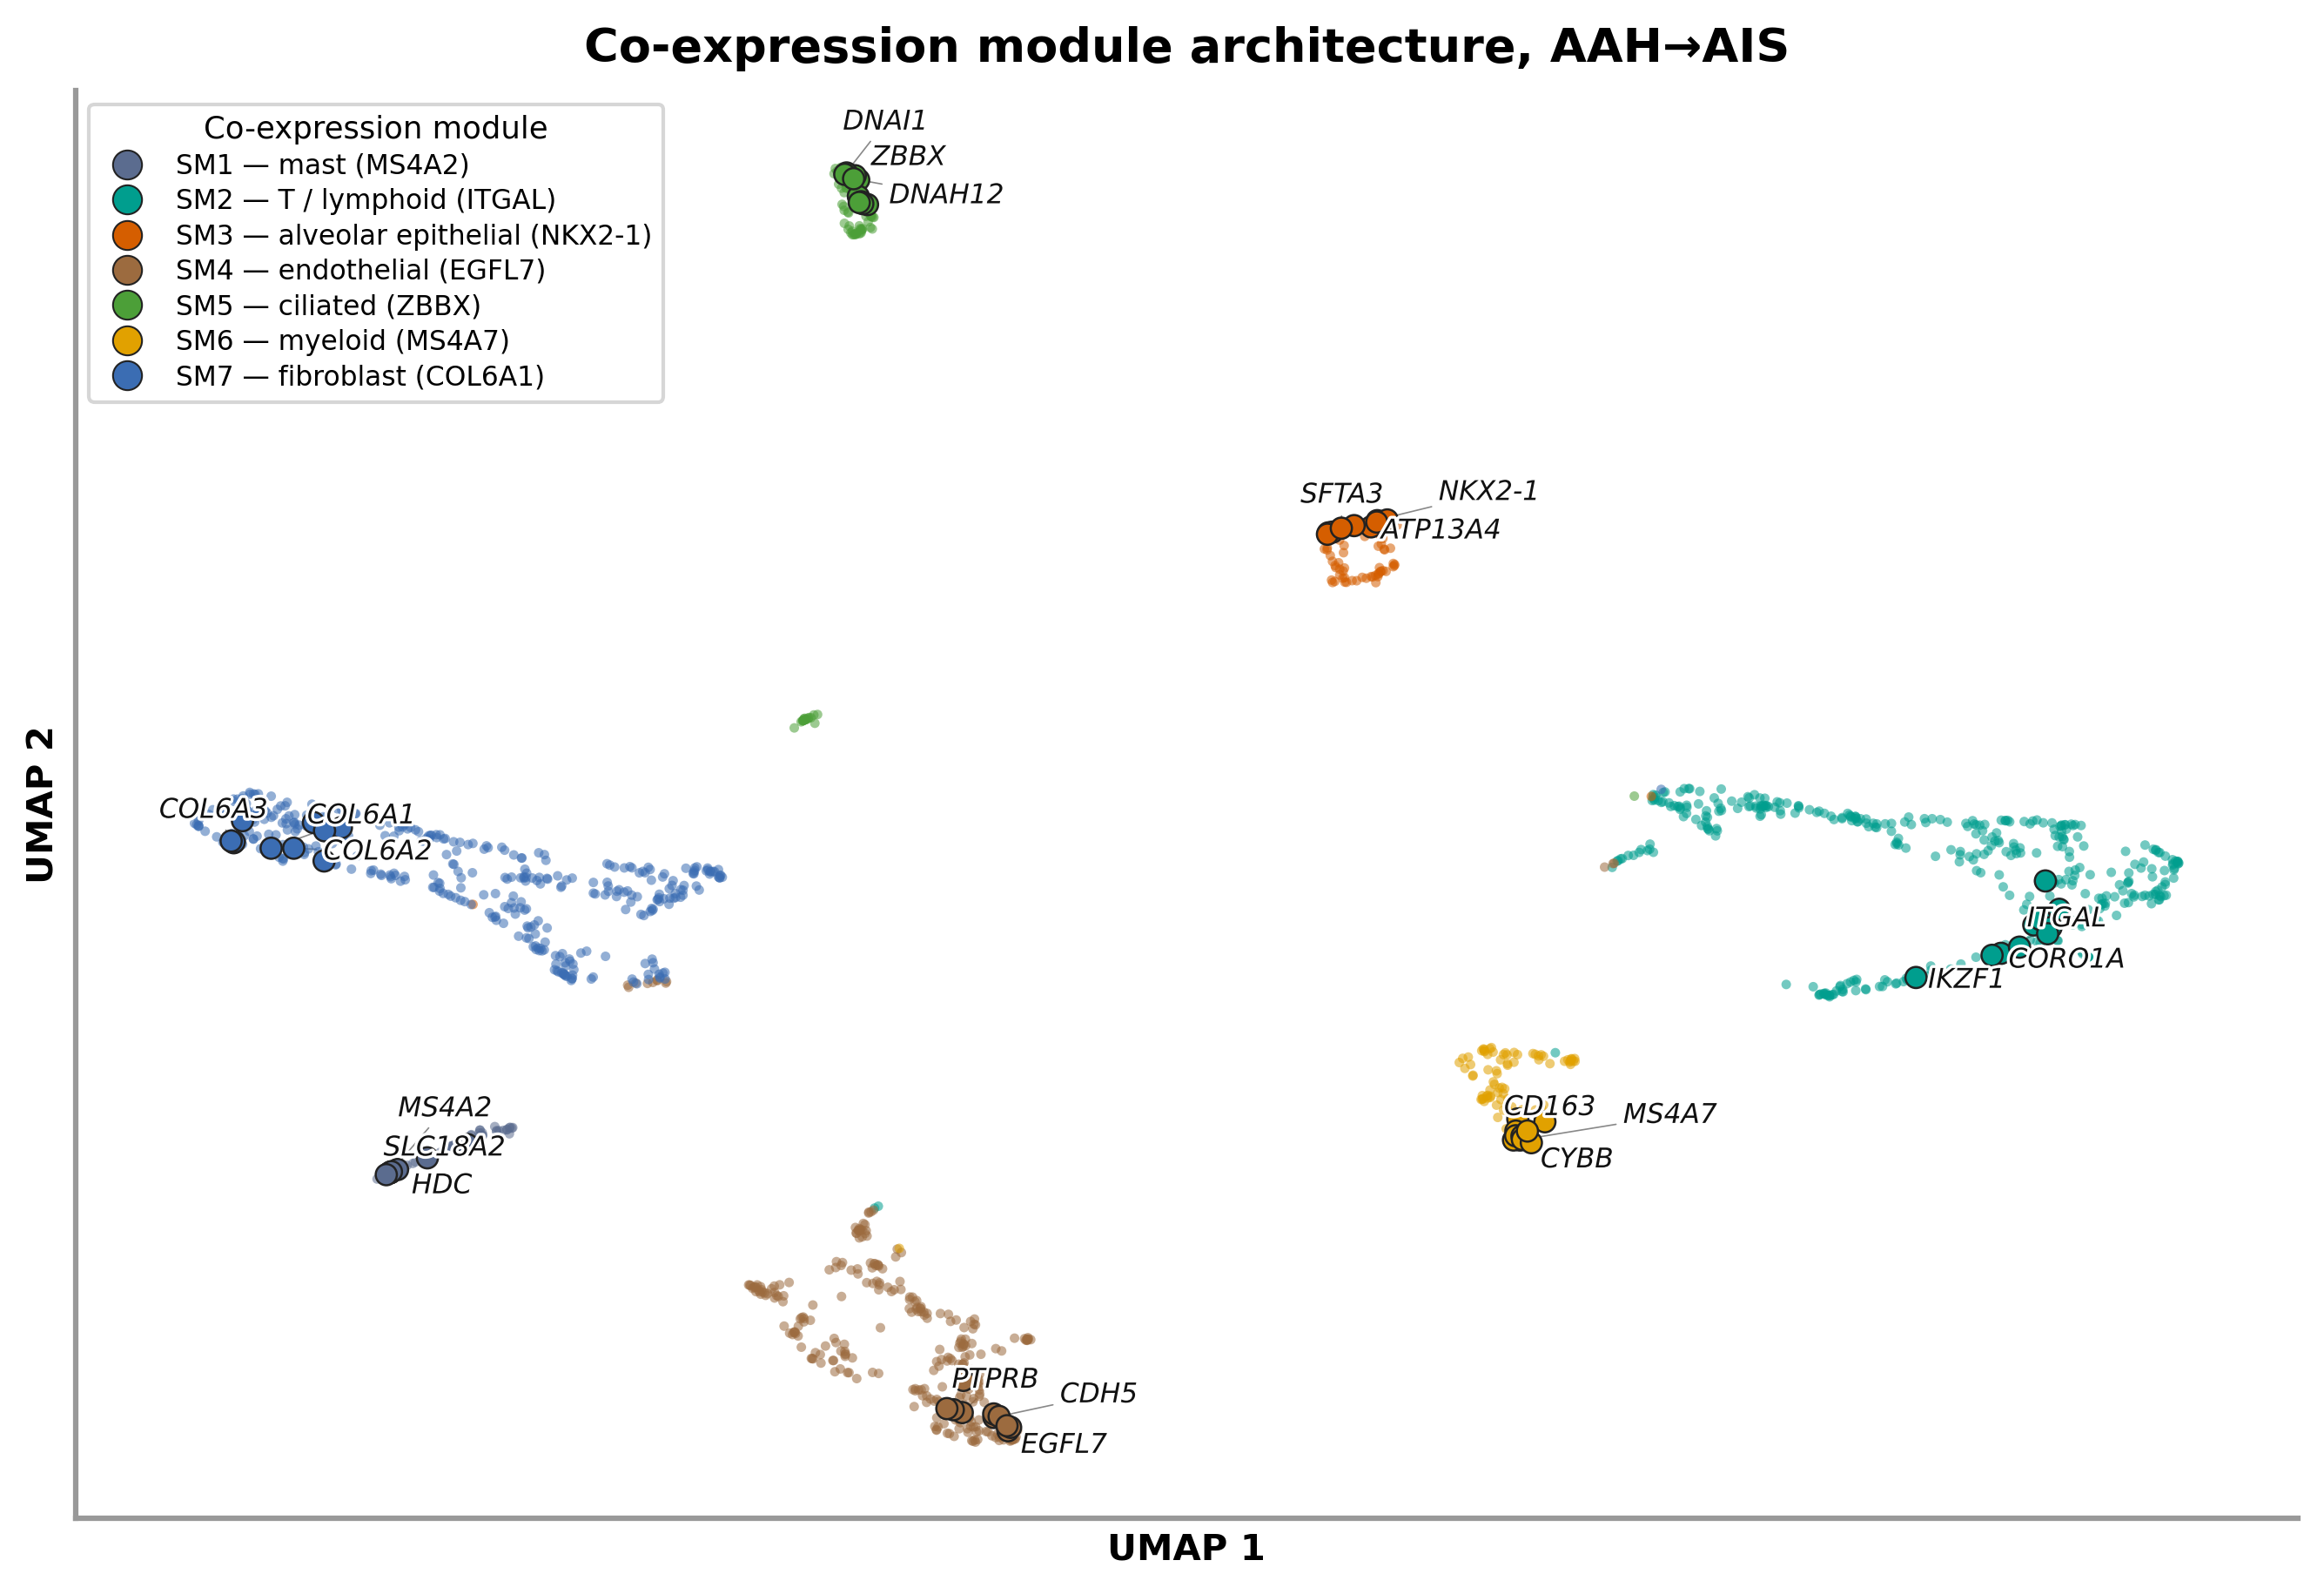
\includegraphics[width=0.92\textwidth]{figures/grn/module_umap_pub_AAH_AIS.png}
  \caption[hdWGCNA co-expression module architecture, AAH$\rightarrow$AIS]{Co-expression module architecture on the AAH$\rightarrow$AIS edge \autocite{Morabito2023-yq}. Genes are embedded on the topological-overlap matrix and colored by module (SM1--SM7); hub genes are ringed and labeled. Modules recover interpretable cell-lineage identities---mast (SM1, MS4A2), T/lymphoid (SM2, ITGAL), alveolar epithelial (SM3, NKX2-1), endothelial (SM4, EGFL7), myeloid (SM6, MS4A7), fibroblast (SM7, COL6A1)---derived purely from co-expression, independent of the CRRT-UDE estimand.}
  \label{fig:module_umap}
\end{figure}

\begin{figure}[htbp]
  \centering
  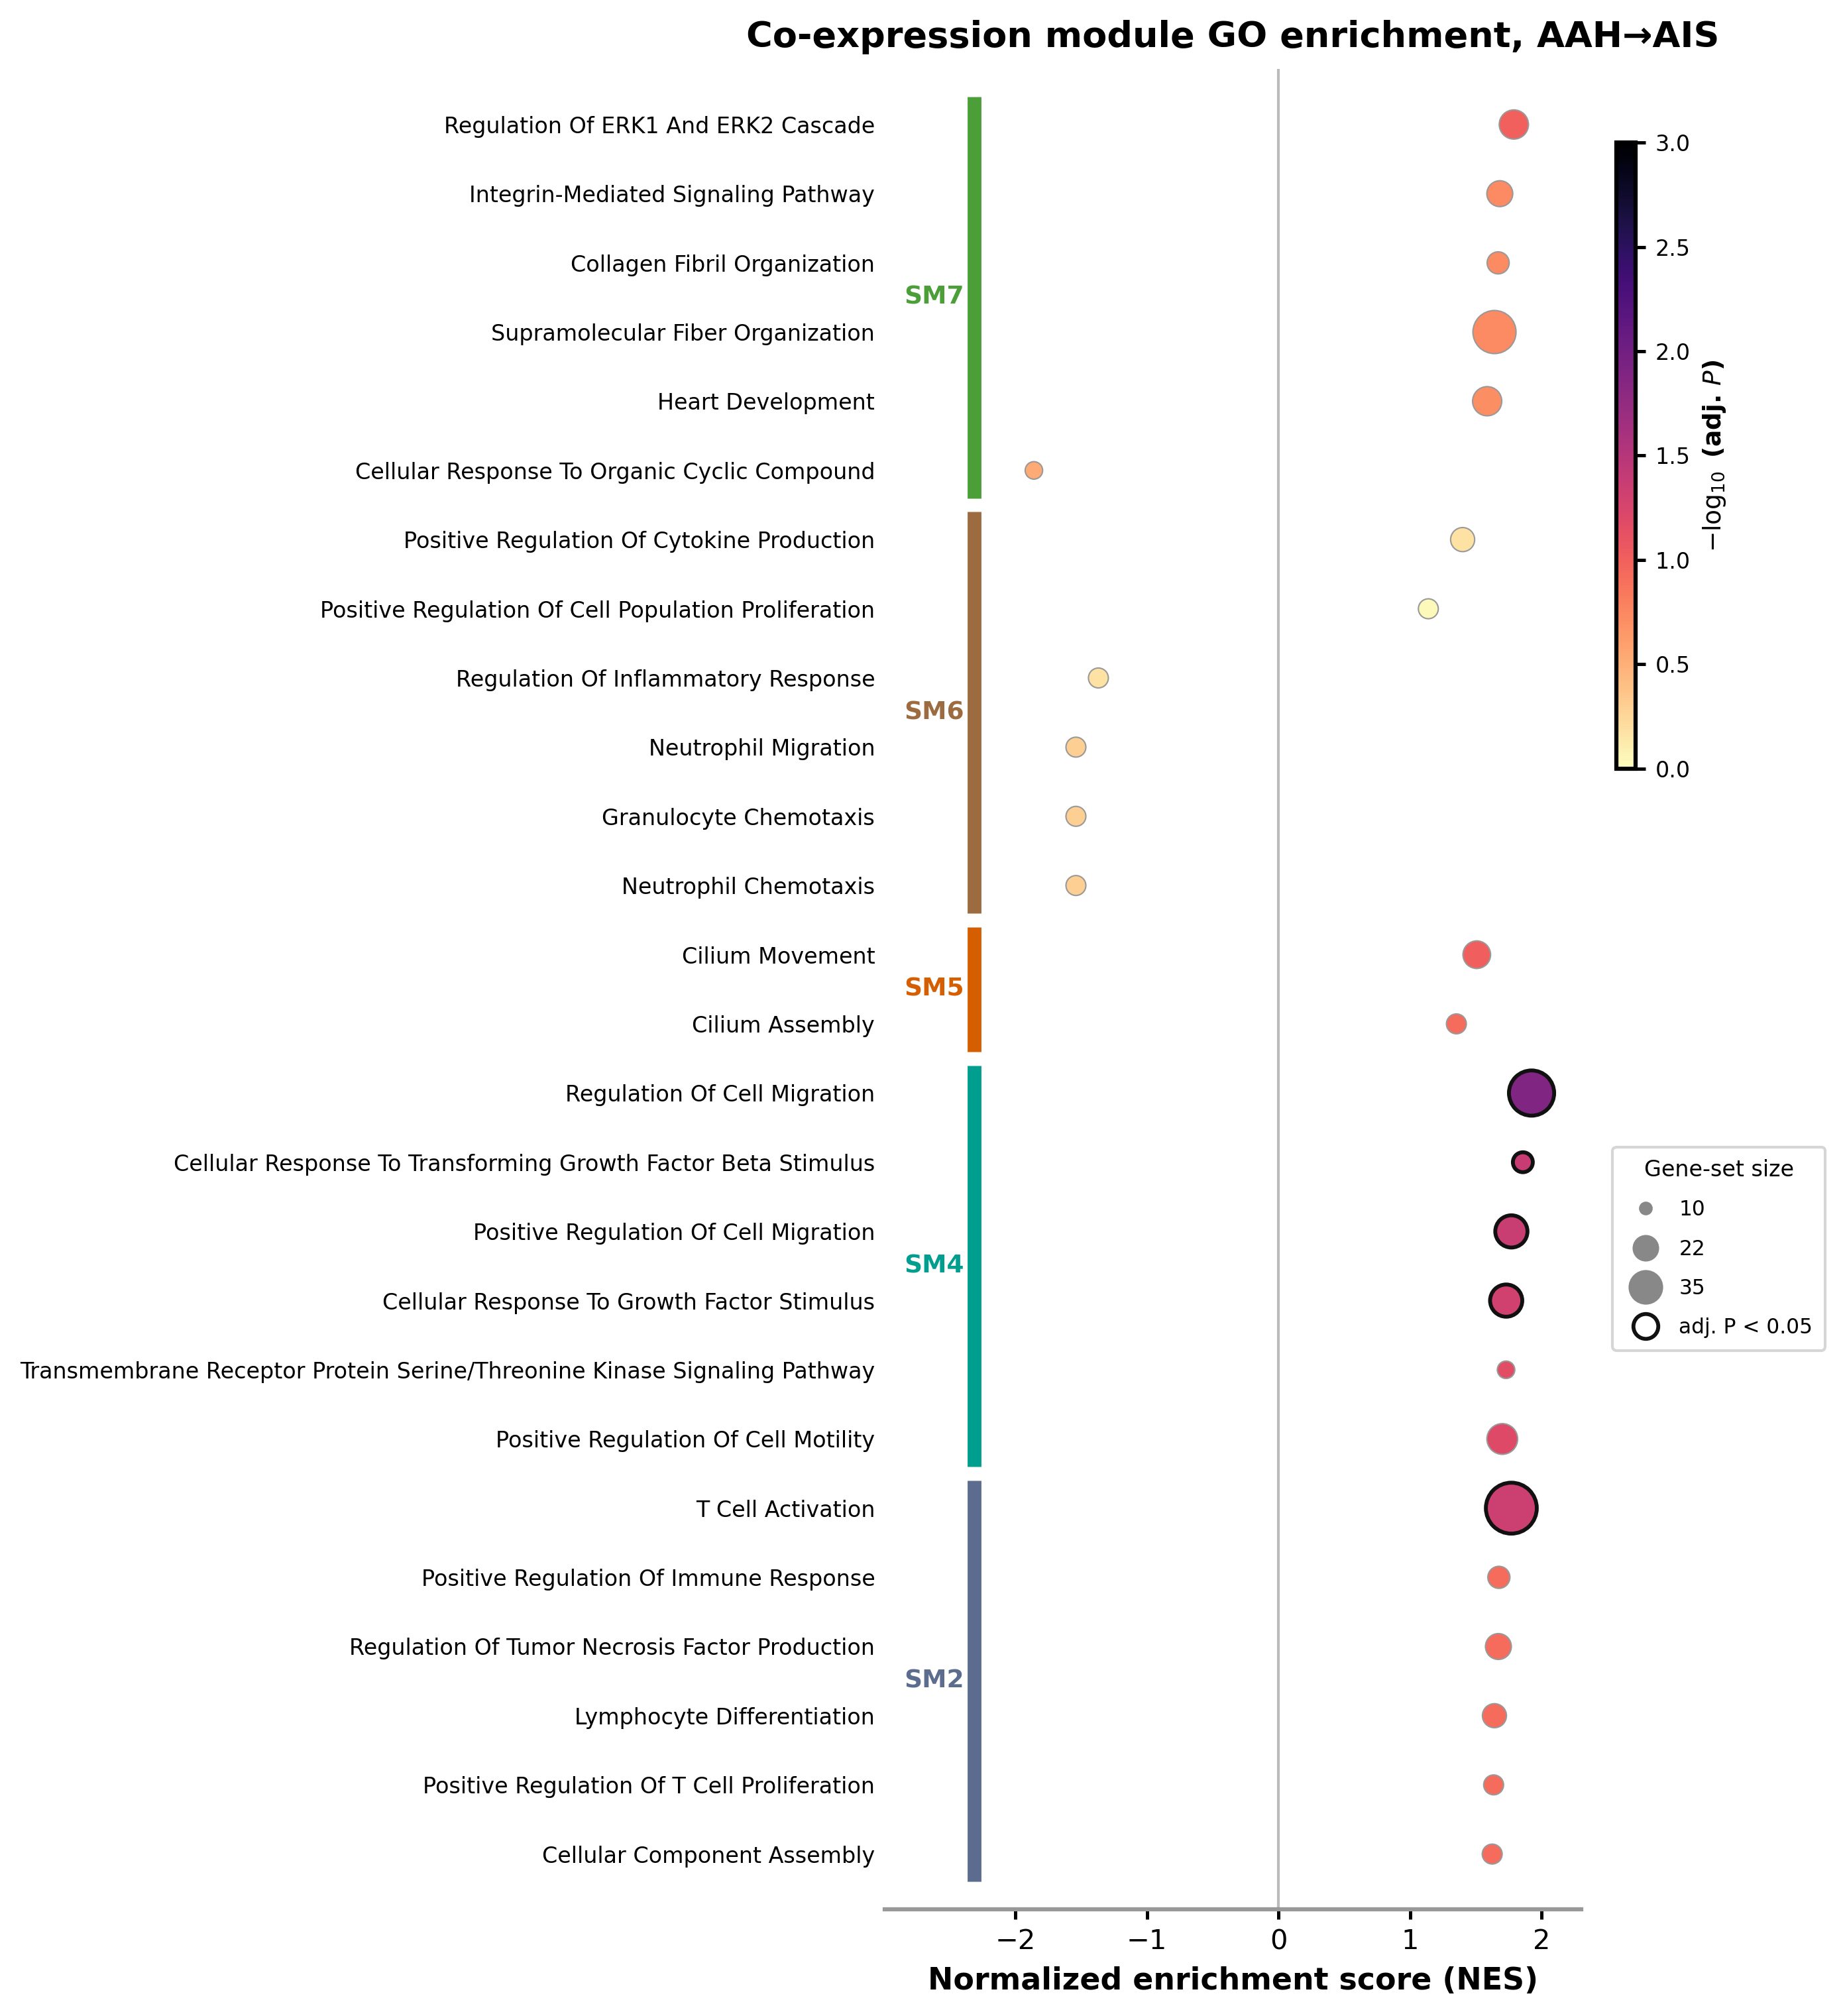
\includegraphics[width=0.95\textwidth]{figures/grn/module_enrichment_AAH_AIS.png}
  \caption[GO-BP enrichment of co-expression modules, AAH$\rightarrow$AIS]{Gene Ontology (Biological Process) enrichment of the hdWGCNA co-expression modules on the AAH$\rightarrow$AIS edge \autocite{Korotkevich2016-ou}. Pathways are grouped by module (colored rail); the $x$-axis is the normalized enrichment score, dot area is gene-set size, and dot color is $-\log_{10}$ adjusted $P$. Terms clearing an adjusted $P<0.05$ are ringed. The vascular/endothelial SM4 module is enriched for regulation of cell migration and TGF$\beta$/MAPK response.}
  \label{fig:module_enrichment}
\end{figure}

\begin{figure}[htbp]
  \centering
  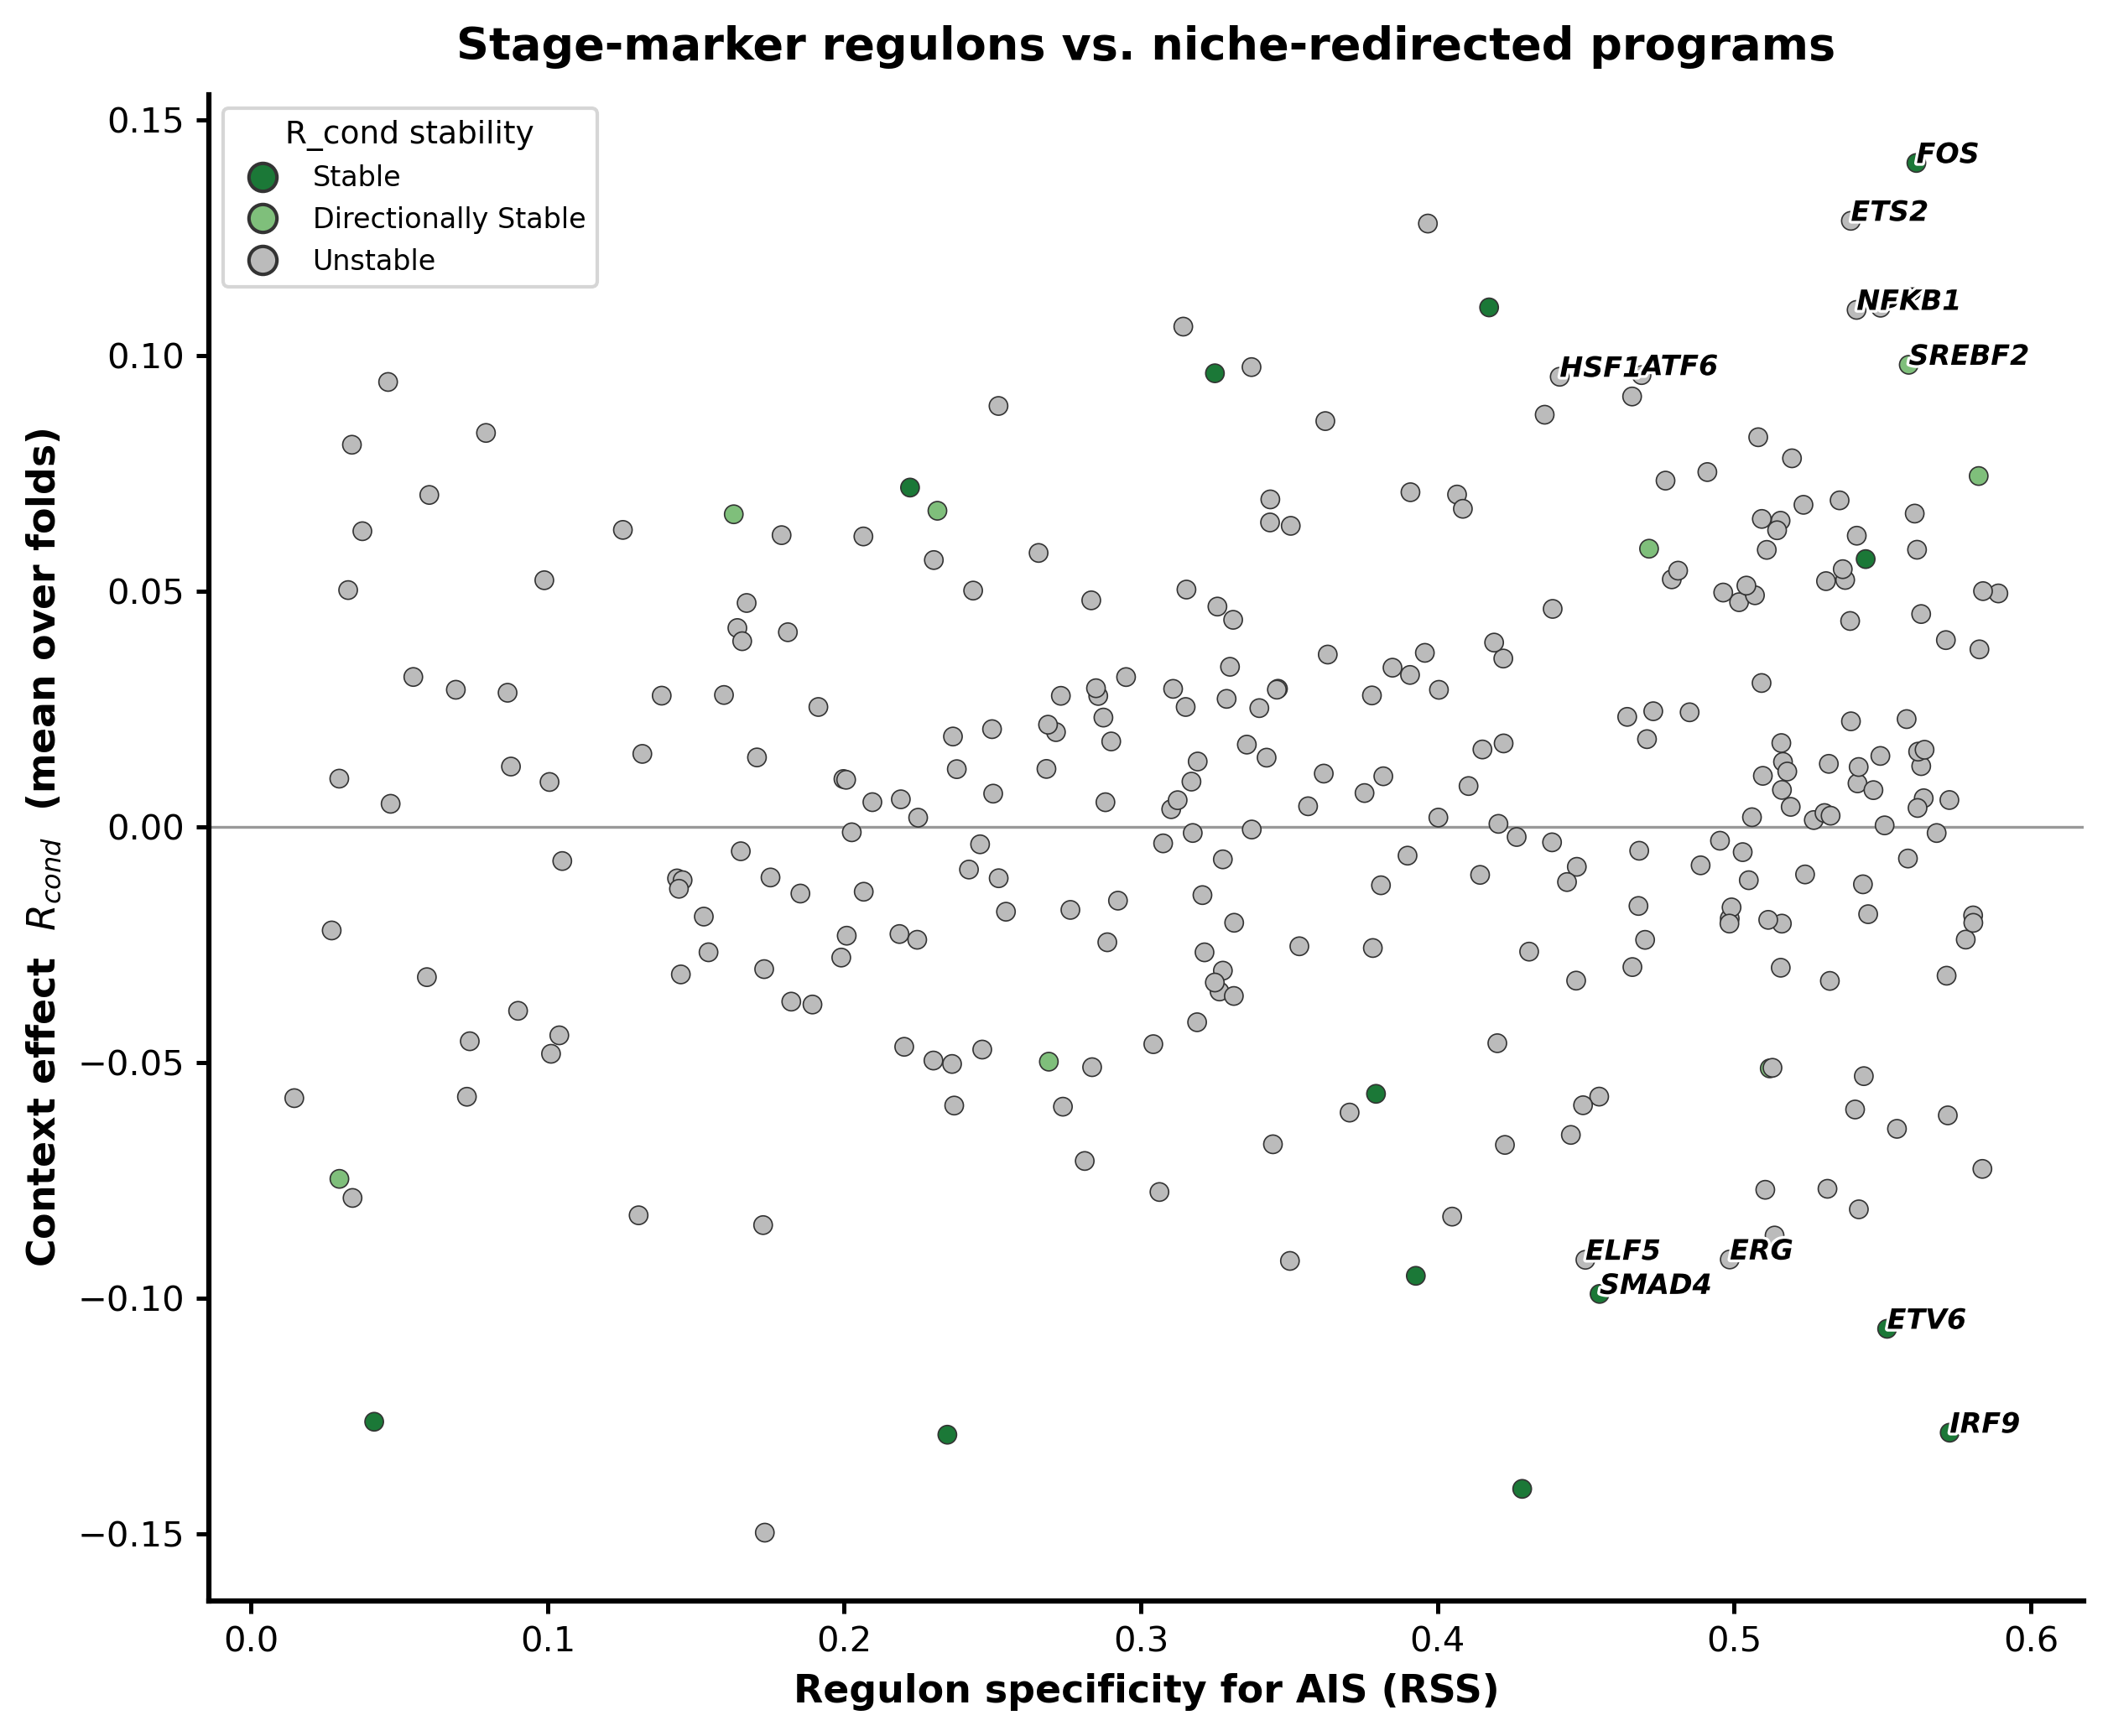
\includegraphics[width=0.95\textwidth]{figures/scenic/scenic_rss_vs_rcond_AAH_AIS.png}
  \caption[Regulon specificity versus context effect, AAH$\rightarrow$AIS]{Each transcription-factor regulon plotted by its stage specificity (regulon specificity score, $x$) against its model context effect ($R_{\text{cond}}$, $y$; mean over folds), colored by $R_{\text{cond}}$ stability. This directly relates the descriptive SCENIC layer to the CRRT-UDE estimand: regulons in the upper-right are both AIS-specific markers and context-upregulated (FOS, ETS2, NF$\kappa$B family), whereas the lower-right marks stage-specific but context-suppressed regulons (IRF9).}
  \label{fig:rss_vs_rcond}
\end{figure}

\begin{figure}[htbp]
  \centering
  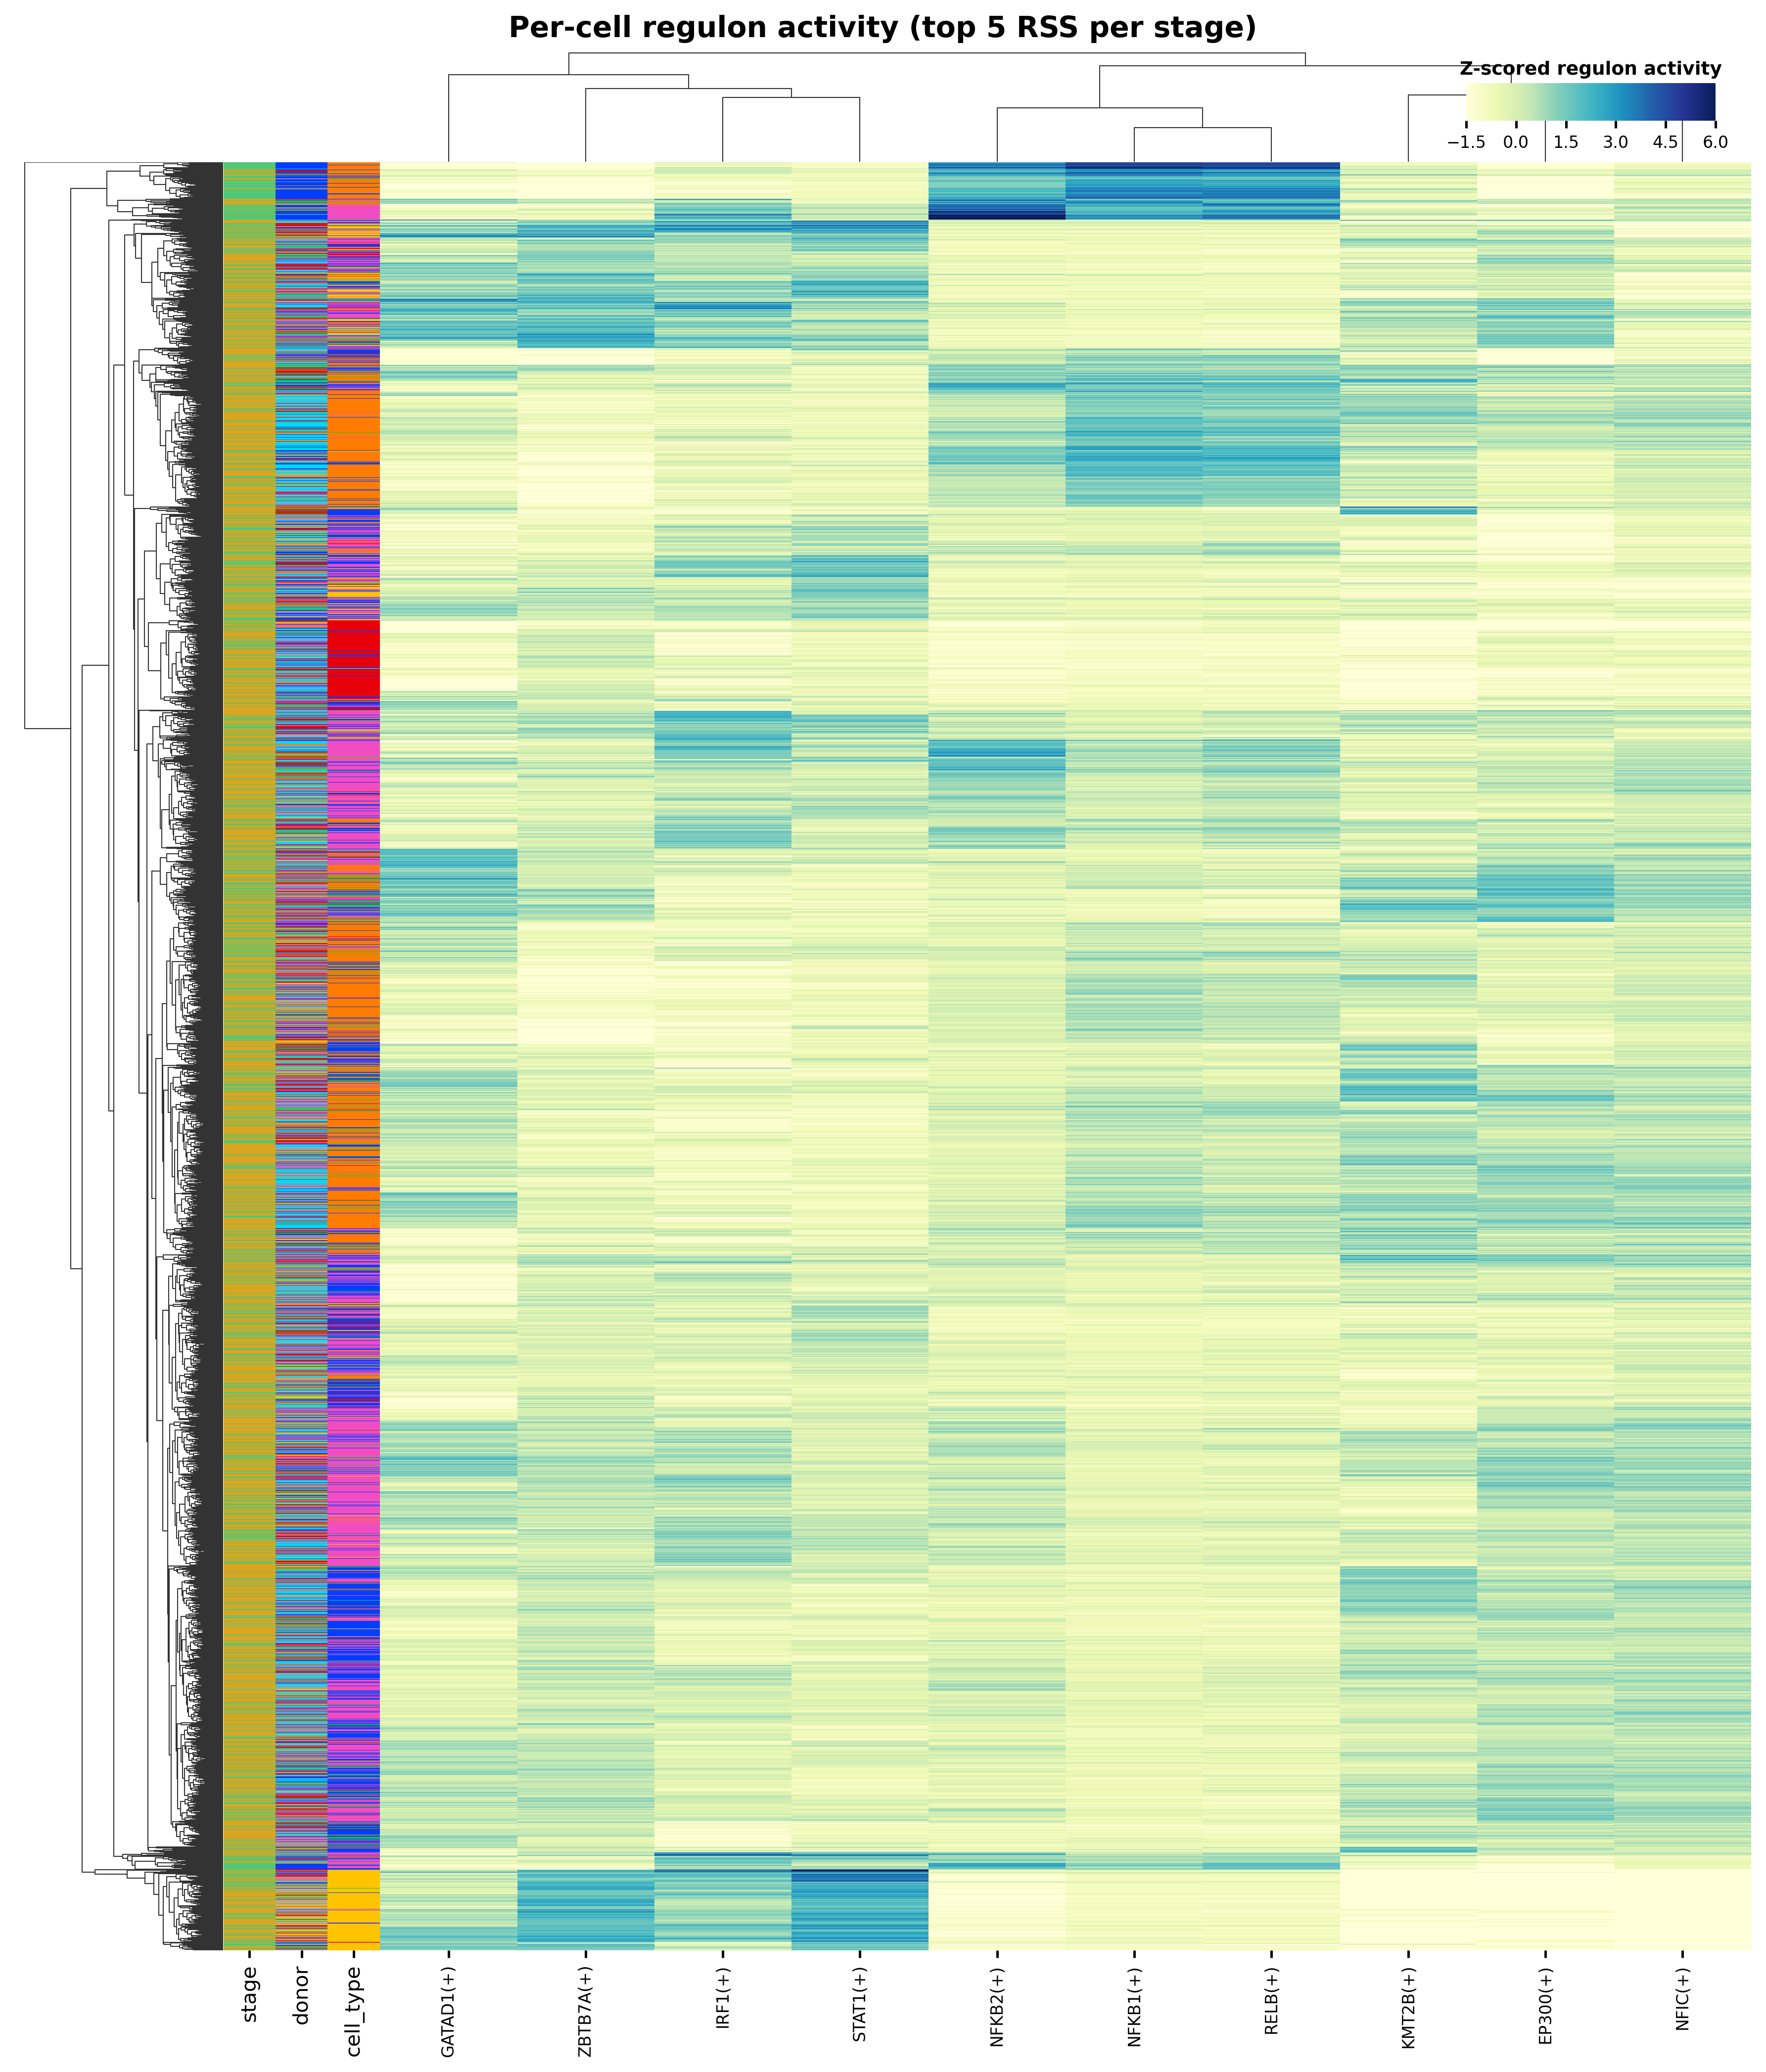
\includegraphics[width=0.95\textwidth]{figures/scenic/scenic_cell_clustermap_AAH_AIS.png}
  \caption[Per-cell regulon-activity clustermap, AAH$\rightarrow$AIS]{Per-cell AUCell regulon-activity clustermap on the AAH$\rightarrow$AIS edge \autocite{Aibar2017-kq}. Rows are individual epithelial cells (hierarchically clustered), columns are the top stage-specific regulons, and color is the $Z$-scored regulon activity. Row-color bars annotate each cell by stage, donor, and dominant cell type, exposing per-patient and per-stage structure. An NF$\kappa$B/STAT/IRF-high inflammatory cell block is visible, consistent with the JAK-STAT and interferon axes identified by $R_{\text{cond}}$.}
  \label{fig:scenic_clustermap}
\end{figure}

% =====================================================================
\section{PanIN supplement}\label{sec:app-c-panin}

The PanIN low-grade$\rightarrow$high-grade edge is a cross-disease transferability and null-calibration
probe and is underpowered by design: it comprises roughly four donors and on the order of one hundred
graded receivers per fold. The per-fold endpoint counts are $53\rightarrow80$ (fold 0, 2 source
donors), $39\rightarrow57$ (fold 1, 1 source donor), and $18\rightarrow22$ (fold 2, 1 source donor).
Of $762$ programs, the powered stability filter returns \emph{zero} STABLE programs; $188$ are
DIRECTIONALLY\_STABLE under a confidence-interval-excludes-zero filter and the remainder are unstable.
This correct-null behavior at this cohort size is the intended calibration result: the estimator does
not manufacture patient-robust stability where the data cannot support it. The largest-magnitude PanIN
programs and their held-out intervals are shown in Figure~\ref{fig:app-c-panin-null}.

\begin{figure}[htbp]
  \centering
  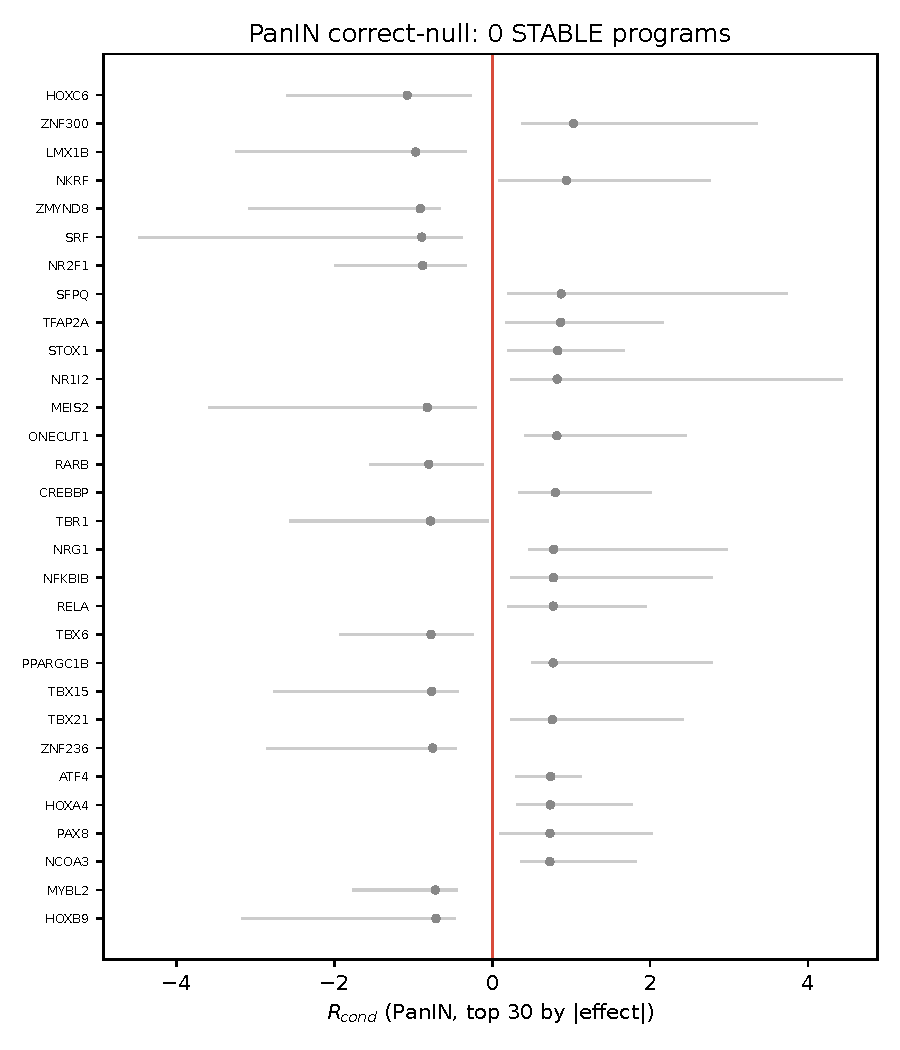
\includegraphics[width=0.6\textwidth]{figures/appendix/panin_null_forest.pdf}
  \caption[PanIN correct-null program forest]{Mean conditional transport $R_{\mathrm{cond}}$ with
  held-out $95\%$ confidence intervals for the $30$ largest-magnitude PanIN low-grade$\rightarrow$high-grade
  programs. No program's interval clears the powered stability filter, so zero programs are classed
  STABLE---the intervals straddle or hug zero as expected under a correctly calibrated null at a
  four-donor cohort size. The estimator does not fabricate patient-robust stability where the data
  cannot support it.}
  \label{fig:app-c-panin-null}
\end{figure} Among the directionally
consistent programs, NF$\kappa$B is context-upregulated ($+0.382$, directionally stable across all
three folds) and EGFR is directionally upregulated ($+0.291$), consistent with an
inflammatory-to-proliferative shift.

The PanIN drift diagnostic is credible in two of three folds ($D_\rho = 1.120$ fold 0,
residual-dominated; $0.820$ fold 1; $0.942$ fold 2). The complete PanIN falsification ladder is
Table~\ref{tab:app-c-ladder-panin}; note that the fold-1 endpoint is dominated by a single-source-donor
split, which inflates every rung on that fold, and that the linear self-only baseline
(\texttt{linear\_baseline\_A}) diverges numerically at this cohort size and is reported in scientific
notation.

\begin{table}[htbp]
  \centering
  \caption[Complete PanIN falsification ladder]{Complete PanIN low-grade$\rightarrow$high-grade
  falsification ladder: per-fold and mean semantic Sinkhorn distance (lower is better), all scored
  rungs, ordered by mean. The three-fold cohort is small and fold 1 (single source donor) inflates
  all rungs.}
  \label{tab:app-c-ladder-panin}
  \footnotesize
  \begin{tabular}{lcccc}
    \toprule
    Ladder rung & Fold 0 & Fold 1 & Fold 2 & Mean \\
    \midrule
    monolithic\_nn & 368.7 & 343.3 & 191.3 & 301.1 \\
    linear\_baseline\_B & 355.5 & 959.4 & 295.8 & 536.9 \\
    neural\_residuals\_only & 398.9 & 1789.2 & 313.8 & 834.0 \\
    spatial\_self\_only & 231.9 & 2926.7 & 222.6 & 1127.0 \\
    strict\_z\_self\_only & 206.6 & 3084.9 & 215.2 & 1168.9 \\
    context\_branch\_only & 392.4 & 2930.5 & 397.4 & 1240.1 \\
    donor\_stage\_average\_context & 265.3 & 3542.3 & 225.0 & 1344.2 \\
    fine\_context\_shuffled\_within\_stratum & 267.4 & 3600.0 & 232.4 & 1366.6 \\
    matched\_state\_shuffled & 376.9 & 3597.8 & 229.1 & 1401.3 \\
    local\_context\_full & 383.9 & 3614.3 & 228.4 & 1408.9 \\
    strict\_z\_full & 220.7 & 4020.9 & 224.0 & 1488.5 \\
    structured\_only & 582.8 & 5854.3 & 409.0 & 2282.0 \\
    one\_step\_full & 352.9 & 11797.3 & 309.7 & 4153.3 \\
    one\_step\_structured\_C & 352.1 & 11810.9 & 309.8 & 4157.6 \\
    linear\_baseline\_A & $4.7\!\times\!10^{4}$ & $6.4\!\times\!10^{5}$ & $1.8\!\times\!10^{7}$ & $6.1\!\times\!10^{6}$ \\
    \bottomrule
  \end{tabular}
\end{table}

% =====================================================================
\section{Software and reproducibility manifest}\label{sec:app-c-software}

The analysis is packaged as the \texttt{crrt-ude} Python package and orchestrated end-to-end with
Snakemake ($\geq 8$) under a SLURM executor. The primary runtime environment
(\texttt{workflow/envs/crrt.yaml}) is Python $3.12$ and includes: numpy, pandas, pyarrow,
scikit-learn, and scipy for numerics; scanpy, anndata ($\geq 0.13$), and squidpy for single-cell and
spatial handling; decoupleR with the PROGENy pathway and CollecTRI transcription-factor priors for
regulatory scoring; scvi-tools for DestVI composition decoding and SCANVI reference surgery against
the LuCA and HLCA atlases; PyTorch, torchdiffeq, POT, and geomloss for the neural fields, RK4
integration, and entropic Sinkhorn transport; liana, omnipath, and GraphRicciCurvature for the
cell--cell communication layer; infercnvpy and PHATE for the malignancy and continuous-geometry
diagnostics; and the \texttt{pybanksy} backend for the Merchavit spatial neighborhood features. The
de-novo corroboration layers (pySCENIC motif-pruned regulons, hdWGCNA weighted co-expression) run in
isolated environments (\texttt{workflow/envs/scclr.yaml}, \texttt{workflow/envs/hdwgcna.yaml}) that
are off the default critical path.

The pipeline configuration is fixed by \texttt{workflow/config.yaml} plus one of the two edge-selector
files. Determinism is anchored by the global seed $0$, with per-component seeds derived from it, and
by patient-held-out folds fit on training donors only. A fully pinned conda lock and a pip freeze are
provided for the SCENIC environment (\texttt{workflow/envs/locks/}); its critical versions are
pySCENIC~$0.12.1$, arboreto~$0.1.6$, ctxcore~$0.2.0$, numpy~$1.23.5$, and pandas~$1.5.3$, allowing exact
recreation of that stage.

The primary transport environment (\texttt{crrt.yaml}) is specified with lower-bound version
constraints rather than exact pins. The core solver stack at analysis time comprised decoupleR,
scvi-tools, PyTorch, torchdiffeq, POT, and geomloss; the byte-exact resolved versions are recorded in
the archived HPC \texttt{conda list} for the analysis environment and are the canonical manifest for
reproduction. All results in this thesis were produced from the \texttt{crrt-ude} repository at commit
\texttt{b350d7d} (branch \texttt{ude-core}, ``source-fixed context is primary
(\texttt{v2lowrank\_source})''), which ties every number in this appendix to an exact revision;
determinism within that revision is anchored by the global seed and patient-held-out folds described
above.



\subsection*{Secondary-analysis parameters}

Chapter~\ref{chap:methods} Section~\ref{sec:methods-biological-analyses} states
what each secondary analysis asks and how its evidential status relates to the
estimand. The settings that reproduce them are collected here.

\small
\setlength{\tabcolsep}{4pt}
\begin{longtable}{@{}>{\raggedright\arraybackslash}p{0.17\textwidth}%
                    >{\raggedright\arraybackslash}p{0.21\textwidth}%
                    >{\raggedright\arraybackslash}p{0.54\textwidth}@{}}
\caption[Secondary-analysis tool settings]{Tool settings for the secondary
biological analyses of Section~\ref{sec:methods-biological-analyses}. All were
run after model fitting and none altered the receiver representation, the
transport coupling, the differential field, or the definition of
$R_{\mathrm{cond}}$.}
\label{tab:app-c-tools}\\
\toprule
Analysis & Tool & Settings \\
\midrule
\endfirsthead
\multicolumn{3}{l}{\small\itshape Table~\ref{tab:app-c-tools} continued from previous page}\\
\toprule
Analysis & Tool & Settings \\
\midrule
\endhead
\midrule
\multicolumn{3}{r}{\small\itshape continued on next page}\\
\endfoot
\bottomrule
\endlastfoot
Stage differential expression & scanpy
  \texttt{rank\_genes\_groups} & Wilcoxon; target stage as comparison group,
  source as reference; signed statistic, log-fold change, nominal and adjusted
  $P$ retained \\
\addlinespace
Gene-set enrichment & decoupleR / fgsea & MSigDB Hallmark and GO Biological
  Process; gene sets with fewer than five ranked genes excluded;
  false-discovery-rate adjustment as returned by the implementation \\
\addlinespace
Stage discrimination & scikit-learn
  \texttt{LogisticRegression} & PROGENy $+$ CollecTRI features only; features
  standardized on training donors; stage-stratified donor-held-out folds, fold
  count limited by the smaller stage-specific donor count; pooled and
  within-donor variants as sensitivity comparisons \\
\addlinespace
Residual localization & scipy \texttt{spearmanr} & Spearman $\rho$ between
  stratum order and per-receiver $R_{\mathrm{cond}}$; $2{,}000$ within-donor
  permutations of stratum labels; two-sided empirical $P$ \\
\addlinespace
Spatial autocorrelation & squidpy
  \texttt{spatial\_neighbors}, \texttt{spatial\_autocorr} & generic coordinate
  type, $k=15$ nearest neighbours, graph built independently per section;
  Moran's $I$ and Getis--Ord $G_i^{\ast}$, hot spots at standardized
  $G_i^{\ast}>1.96$ and cold spots below $-1.96$; section-level Spearman,
  Kruskal--Wallis, and two-sided Mann--Whitney $U$ across stages \\
\addlinespace
Projected dynamics & PHATE (primary), UMAP, PCA & velocities from the first
  displacement of a multistep RK4 trajectory, projected into the shared
  embedding and smoothed on a regular grid; spectral Helmholtz--Hodge
  decomposition; rotational fraction as the rotational-component norm over the
  full projected-field norm \\
\addlinespace
Regulon inference & pySCENIC & GRNBoost2 co-expression on raw epithelial
  counts; cisTarget motif pruning; AUCell per-nucleus activity; overlap with
  $R_{\mathrm{cond}}$ transcription factors by upper-tail hypergeometric test on
  a universe restricted to factors present in both \\
\addlinespace
Co-expression modules & hdWGCNA & metacells within compatible donor, stage, and
  cell-type groups; topological-overlap matrix from the selected
  soft-thresholding power; hierarchical clustering with dynamic tree cutting;
  modules merged on eigengene correlation; hub genes by intramodular
  connectivity and eigengene membership \\
\addlinespace
Communication & LIANA, OmniPath, CollecTRI & LIANA consensus per stage;
  receptor-to-transcription-factor paths from OmniPath directed interactions;
  chains retained only where the terminal program is stable or directionally
  stable with $|R_{\mathrm{cond}}|\geq0.05$; Ollivier--Ricci curvature for
  bottleneck ranking, exploratory \\
\end{longtable}